\documentclass[a4paper]{report}
\usepackage[utf8]{inputenc}
\usepackage[portuguese]{babel}
\usepackage{hyperref}
\usepackage{a4wide}
\hypersetup{pdftitle={CG - Fase 2 - Grupo 7},
pdfauthor={João Teixeira, José Ferreira, Miguel Solino},
colorlinks=true,
urlcolor=blue,
linkcolor=black}
\usepackage{subcaption}
\usepackage[cache=false]{minted}
\usepackage{listings}
\usepackage{booktabs}
\usepackage{multirow}
\usepackage{appendix}
\usepackage{tikz}
\usepackage{authblk}
\usepackage{bashful}
\usepackage{verbatim}
\usepackage{amsmath}
\usepackage{tikz}
\usepackage{tikz,fullpage}
\usepackage{pgfgantt}
\usepackage{amssymb}
\usepackage{mwe}
\usetikzlibrary{arrows,%
                petri,%
                topaths}%
\usepackage{tkz-berge}
\usetikzlibrary{positioning,automata,decorations.markings}
\AfterEndEnvironment{figure}{\noindent\ignorespaces}
\AfterEndEnvironment{table}{\noindent\ignorespaces}

\definecolor{solarized@base03}{HTML}{002B36}
\definecolor{solarized@base02}{HTML}{073642}
\definecolor{solarized@base01}{HTML}{586e75}
\definecolor{solarized@base00}{HTML}{657b83}
\definecolor{solarized@base0}{HTML}{839496}
\definecolor{solarized@base1}{HTML}{93a1a1}
\definecolor{solarized@base2}{HTML}{EEE8D5}
\definecolor{solarized@base3}{HTML}{FDF6E3}
\definecolor{solarized@yellow}{HTML}{B58900}
\definecolor{solarized@orange}{HTML}{CB4B16}
\definecolor{solarized@red}{HTML}{DC322F}
\definecolor{solarized@magenta}{HTML}{D33682}
\definecolor{solarized@violet}{HTML}{6C71C4}
\definecolor{solarized@blue}{HTML}{268BD2}
\definecolor{solarized@cyan}{HTML}{2AA198}
\definecolor{solarized@green}{HTML}{859900}

\lstset{
  language=Java,
  upquote=true,
  columns=fixed,
  tabsize=4,
  extendedchars=true,
  breaklines=true,
  numbers=left,
  numbersep=5pt,
  rulesepcolor=\color{solarized@base03},
  numberstyle=\tiny\color{solarized@base01},
  basicstyle=\footnotesize\ttfamily,
  keywordstyle=\color{solarized@green},
  stringstyle=\color{solarized@yellow}\ttfamily,
  identifierstyle=\color{solarized@blue},
  commentstyle=\color{solarized@base01},
  emphstyle=\color{solarized@red}
}

\begin{document}

\title{Computação Gráfica\\
\large Fase 2 - Grupo 7}
\author{José Ferreira (A83683) \and João Teixeira (A85504) \and Miguel Solino (A86435)}
\date{\today}

\begin{center}
    \begin{minipage}{0.75\linewidth}
        \centering
        
\includegraphics[width=0.4\textwidth]{images/eng.jpeg}\par\vspace{1cm}
        \vspace{1.5cm}
        \href{https://www.uminho.pt/PT}
        {\color{black}{\scshape\LARGE Universidade do Minho}} \par
        \vspace{1cm}
        \href{https://www.di.uminho.pt/}
        {\color{black}{\scshape\Large Departamento de Informática}} \par
        \vspace{1.5cm}
        \maketitle
    \end{minipage}
\end{center}

\tableofcontents

\chapter{Introdução}
Este trabalho foi desenvolvido no âmbito da unidade curricular de computação
gráfica e está dividido em várias fases de entrega distintas sendo que esta é a
segundo.\\
Ao longo desta fase dividimos o trabalho em 4 partes:
Primeiro melhoramos o parser de xml desenvolvido na fase anterior de forma a
suportar operações de openGl. Depois melhoramos algumas funcionalidades do
engine em si. Por fim, tal como foi pedido, desenvolvemos uma scene que
representa o nosso sistema solar com recurso a um script em Python.\\
Enquanto fizemos o sistema solar reparamos que precisávamos de uma forma de
desenhar aneís em planetas que o tivéssemos. A forma mais fácil
de implementar isso seria recorrendo a uma Torus espalmada, ou seja, com um
scale no eixo do Y com um valor muito próximo de 0. Assim, também implementamos
mais uma primitiva, a Torus.
Ao longo deste relatório irá ser explicado a metodologia e raciocínio usados
para a realização desta fase.\\

\chapter{Engine}
Neste módulo foi desenvolvido um motor 3D simples.\\
Quando se executa o programa gerado por defeito é aberta a scene guardada em
\textit{scenes/config.xml}. Se alguém ficheiro for passado como argumento esse
será o selecionado.\\

\section{XML parsing}
Para dar parsing ao XML utilizamos a biblioteca \textit{TinyXML}.\\
Visto que é necessário que o ficheiro seja lido apenas uma vez é necessário
criar uma estrutura para armazenar os dados contidos no XML. Visto que estes se
assemelham a uma árvore decidimos criar uma classe recursiva chamda Group que
representa cada nó dessa árvore.\\
Esta classe contém um vetor de transformações, um vetor de modelos, a cor que
foi definida nesse nodo (ou, se nenhuma foi definida, a cor do nodo pai) e um
vetor de Group filhos.\\
Esta classe te, dois construtores definidos. Um que recebe todos os parametros
referidos acima e um que recebe o caminho para o ficheiro XML a ler.\\
Assim, para ler um ficheiro para memória e guardar num singleton basta fazer.

\begin{lstlisting}
group = Group(sceneName);
\end{lstlisting}
Quando esta função é chamada primeiro o ficheiro é aberto, e obtém-se o nodo
base do ficheiro com recurso ao \textit{TinyXML} e com o devido error
checking.\\
Depois chama-se a função auxiliar, Parser, que está preparada para dar parse a
cada nodo do XML.

\begin{lstlisting}
Group::Group(const char *fileName) {
  TiXmlDocument doc(fileName);
  if (!doc.LoadFile()) {
    throw doc.ErrorDesc();
  }

  TiXmlElement *root = doc.FirstChildElement();
  if (!root) {
    throw "Failed to load file: No root element.";
  }

  *this = Parser(doc.FirstChildElement(), Colour());
}
\end{lstlisting}
De forma a extrair todos os dados necessários de cada nodo a função Parser
percorre todos os nodos filho do nodo que se está a analizar.\\
Assim, se o nodo filho tiver um valor de translate, rotate ou scale é convertido
numa transformação e colocado no vetor de transformações \textit{vTran}. De
forma a permitir que apenas os valores pretendidos sejam preenchidos nas
transformações implementamos valores \textit{default}.\\
Se o nodo tiver o valor de model é lido o nome do ficheiro dos atributos e é
criado um Model que recebe o nome do ficheiro e a cor currente e é adicionado ao
vetor \textit{vMod}.\\
Por fim, para qualquer outro nodo, é tratado como um Group filho e a função
parser é chamada recursivamente, sendo que o resultado desta função é adicinado
ao vetor \textit{vGroup}.\\
Assim já temos todos os elementos para criar um Group que é criado e
desenvolvido.

\begin{lstlisting}
Group Parser(TiXmlElement *root, Colour colour) {
  std::vector<Transform> vTran;
  std::vector<Model> vMod;
  std::vector<Group> vGroup;

  for (TiXmlElement *elem = root->FirstChildElement(); elem != NULL;
       elem = elem->NextSiblingElement()) {
    std::string_view type = elem->Value();

    if (type == "translate") {
      float x = std::stof(elem->Attribute("X") ?: "0");
      float y = std::stof(elem->Attribute("Y") ?: "0");
      float z = std::stof(elem->Attribute("Z") ?: "0");
      vTran.push_back(Translate(x, y, z));
    } else if (type == "rotate") {
      float ang = std::stof(elem->Attribute("angle") ?: "0");
      float x = std::stof(elem->Attribute("axisX") ?: "0");
      float y = std::stof(elem->Attribute("axisY") ?: "0");
      float z = std::stof(elem->Attribute("axisZ") ?: "0");
      vTran.push_back(Rotate(ang, x, y, z));
    } else if (type == "scale") {
      float x = std::stof(elem->Attribute("X") ?: "1");
      float y = std::stof(elem->Attribute("Y") ?: "1");
      float z = std::stof(elem->Attribute("Z") ?: "1");
      vTran.push_back(Scale(x, y, z));
    } else if (type == "model") {
      vMod.push_back(
          Model(elem->Attribute("file"), parse_colour(elem, colour)));
    } else {
      vGroup.push_back(Parser(elem, parse_colour(elem, colour)));
    }
  }
  return Group(std::move(vTran), std::move(vMod), colour, std::move(vGroup));
}
\end{lstlisting}
Para desenhar o Group criado basta aplicar todas as tranformações definidas no
vetor, desenhar todos os modelos definidos e por fim chamar recursivamente a
função para desenhar sobre os subgrupos.

\begin{lstlisting}
void Group::draw_group() const {
  for (auto const &t : transformations)
    t.apply();
  for (auto const &m : models)
    m.draw_model();
  for (auto const &g : subgroups) {
    glPushMatrix();
    g.draw_group();
    glPopMatrix();
  }
}
\end{lstlisting}

\subsection{Extensões de XML implementadas}
Para além das funcionalidades pedidas no enunciado também implementamos a
possibilidade de indicar a cor que se pretende desenhar.\\
De forma a facilitar a escrita das cores decidimos utilizar a sintaxe de
\#RRGGBB
e \#RRGGBBAA. E esta pode facilmente ser definida em qualquer label que não
represente uma transformação. Assim, é possível definir a cor no group (fazendo
que com todos os modelos e subgrupos tenham a mesma cor) ou dentro do models
(fazendo com que todos os subgroups e modelos tenham a mesma cor)
Por exemplo,
\begin{lstlisting}
<scene>
    <!-- group 1 -->
    <group colour="#FF0000">
        <models>
            <model file="models/sphere.3d" />
        </models>
        <!-- subgroup 1 -->
        <group>
            <translate Y=2 />
            <models>
                <model file="models/cone.3d" />
            </models>
        </group>
        <!-- subgroup 2 -->
        <group colour="#00FF00">
            <translate Y=-1 />
            <models>
                <model file="models/torus.3d" />
            </models>
        </group>
    </group>
</scene>
\end{lstlisting}
\begin{figure}[H]
    \centering 
    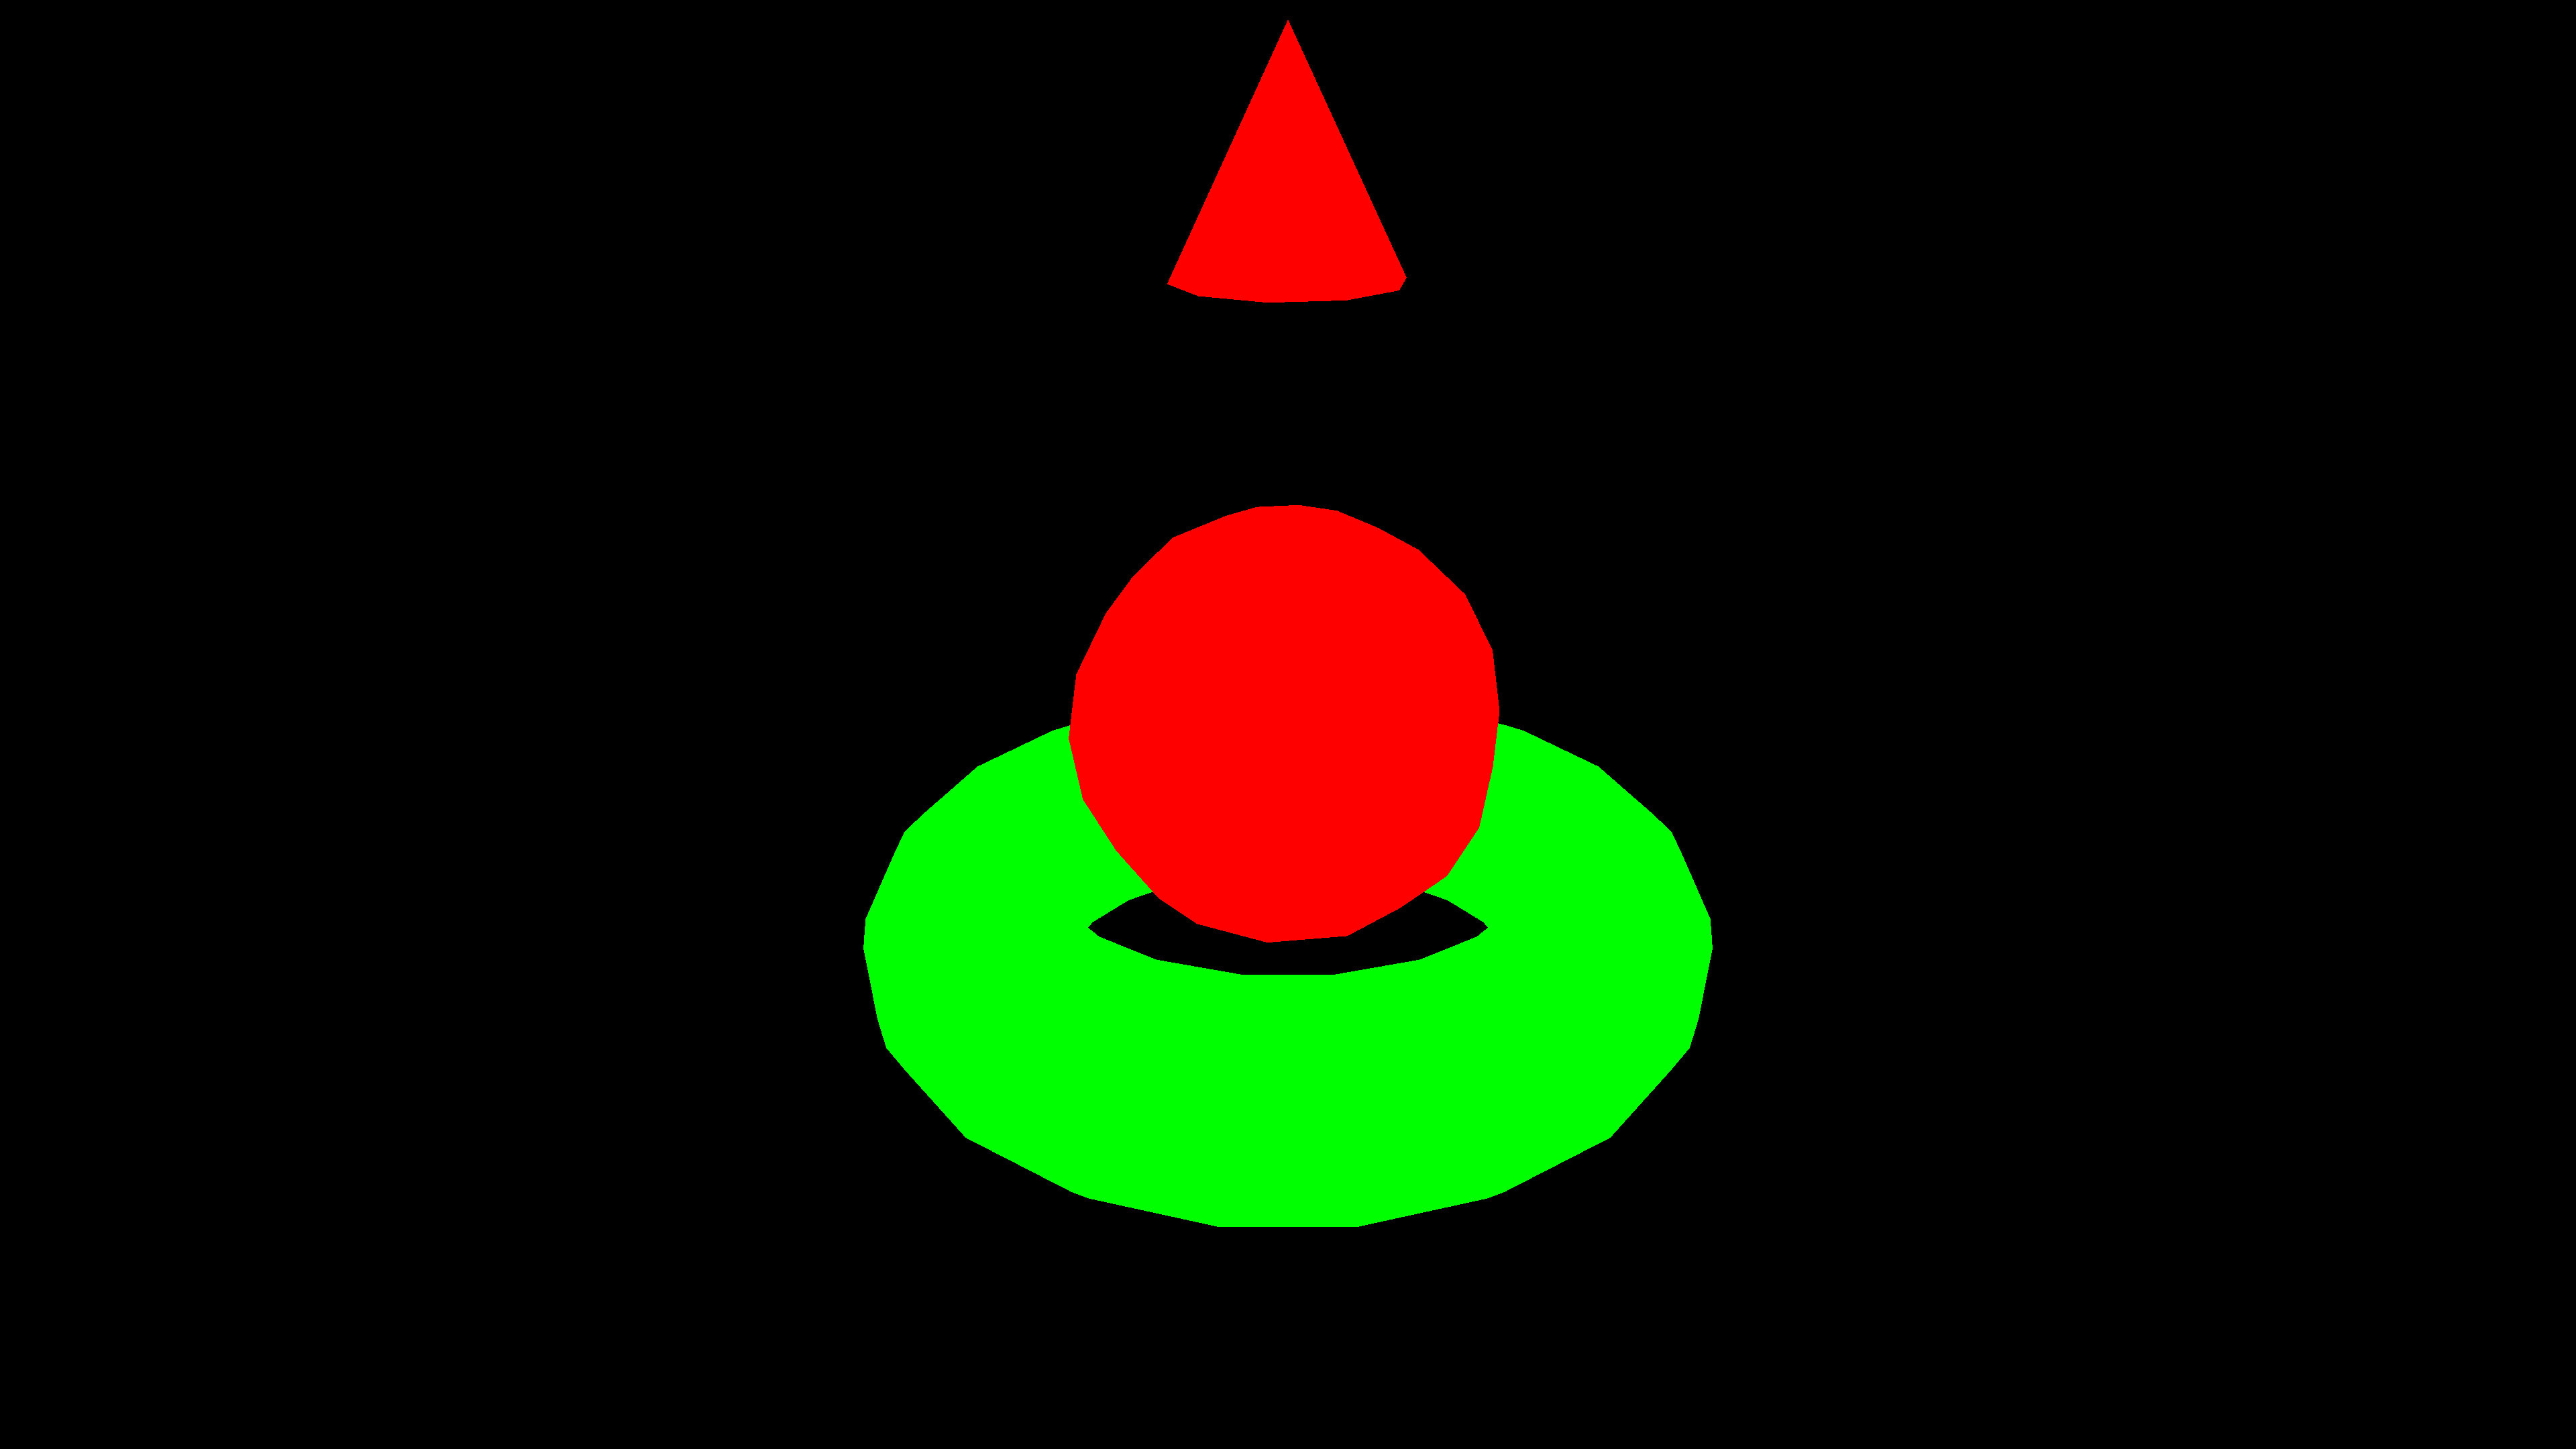
\includegraphics[width=0.5\textwidth]{images/example.png}
    \caption{Exemplo no engine}
    \label{fig:scheme_torus}
\end{figure}
Neste exemplo, tanto o subgroup 1 como o subgroup 2 herdam a cor definida no
group 1. No entanto como o subgroup 2 tem uma cor definida dentro os models
definidos dentro desse têm essa cor.

\section{Camera}
\subsection{Moving the Camera}
Para mover a camera são usados dois keysets. O WASD é usado para mover o ponto
para onde a camera está a olhar (\textit{\_center}). o HJKL é usado para orbitar
esse ponto (\textit{\_pl}).\\
Para desenhar a camera basta usar a função \textit{gluLookAt}.
\begin{lstlisting}
gluLookAt(_pl.x(),_pl.y(),_pl.z(), 
	_center.x(),_center.y(),_center.z(),
		0.0f,1.0f,0.0f);
\end{lstlisting}
Para mover a camera definimos um vetor que vai de um ponto para o outro.\\
Assim, para fazer as operações sobre a camera utilizamos as as funções definidas
na classe \textit{Point} aliadas ao vetor calculado anteriormente.\\
Por exemplo, para mover a camera e o ponto para onde se está a olhar para a
frente relativamente à direção para que a camera está a olhar.\\
Primeiro é calculado um vetor paralelo ao plano XZ alinhado com o vetor
calculado mas no sentido contrário e de comprimento 0.1. Agora basta somar esse
vetor aos pontos da classe.\\
\begin{lstlisting}
t = VectorSpherical(0.1, M_PI / 2, v.azimuth() + M_PI);
_pl = _pl + t;
_center = _center + t;
\end{lstlisting}

\subsection{Special Keybinds}
\begin{itemize}
    \item \textbf{x}: toggles eixos
        \begin{figure}[H]
            \centering
            \begin{minipage}{0.49\textwidth}
                \centering
                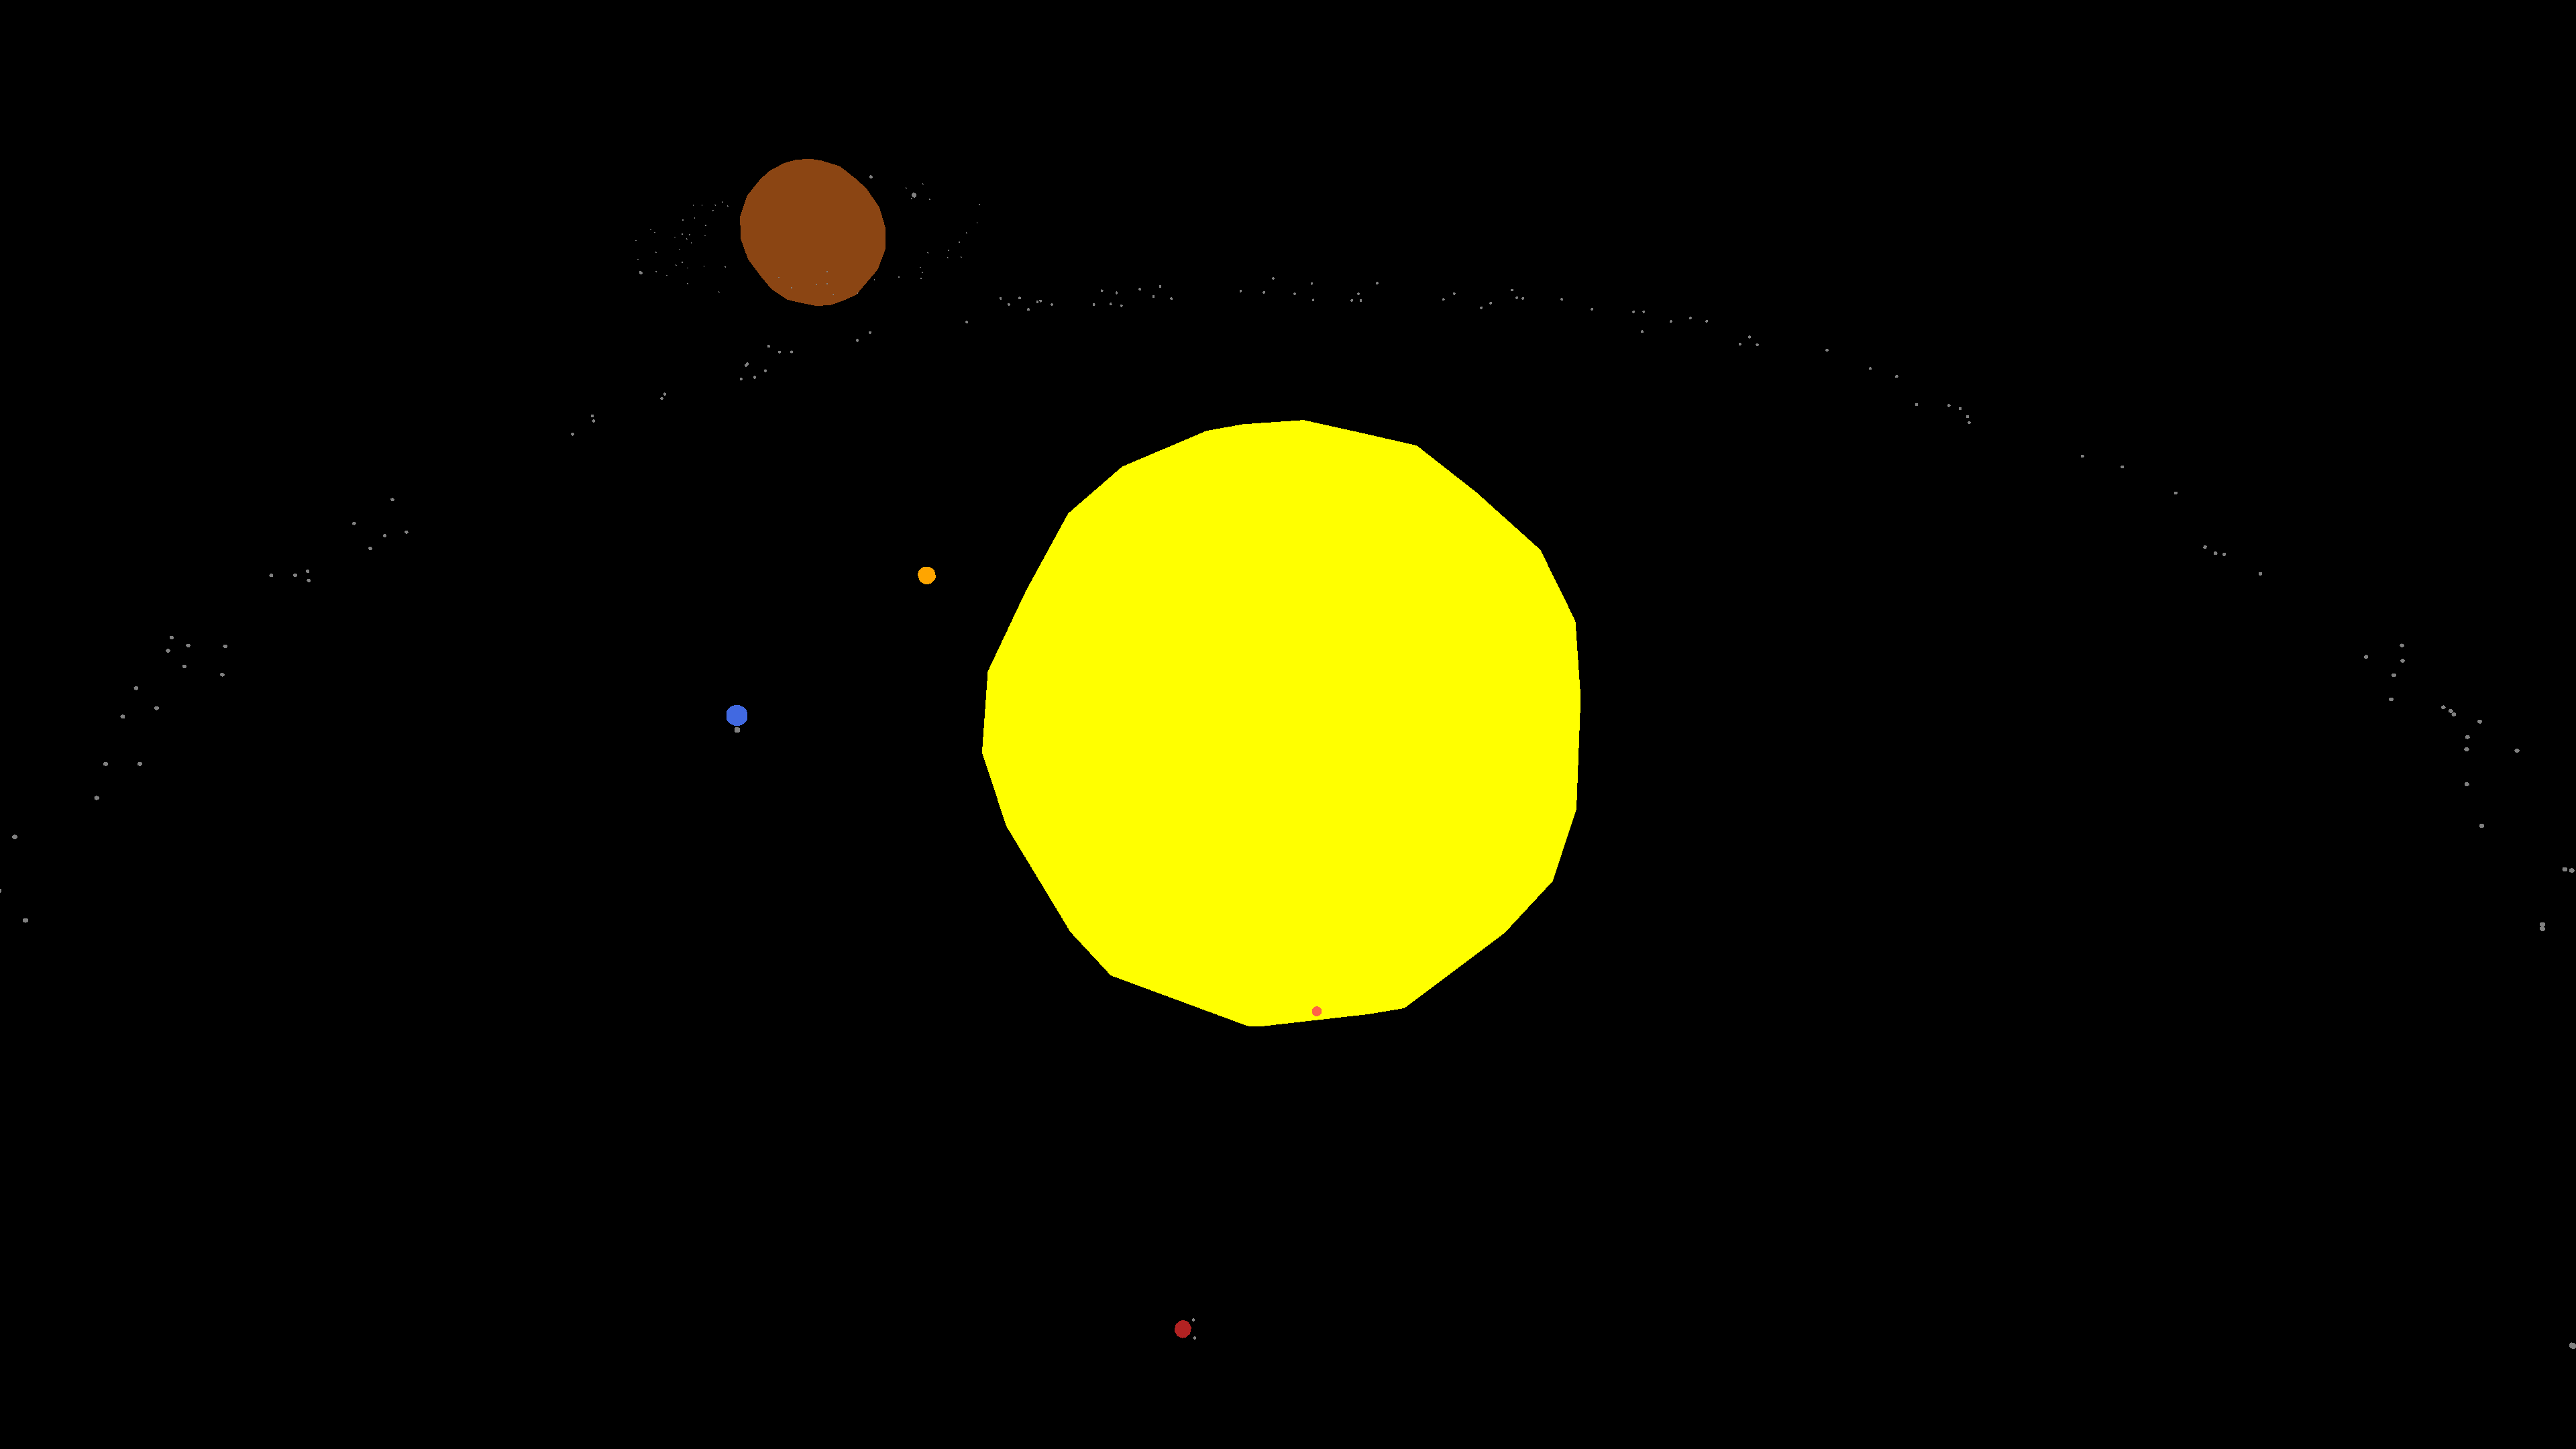
\includegraphics[width=\textwidth]{images/no_axis.png}
                \caption{sem eixos}
            \end{minipage}\hfill
            \begin{minipage}{0.49\textwidth}
                \centering
                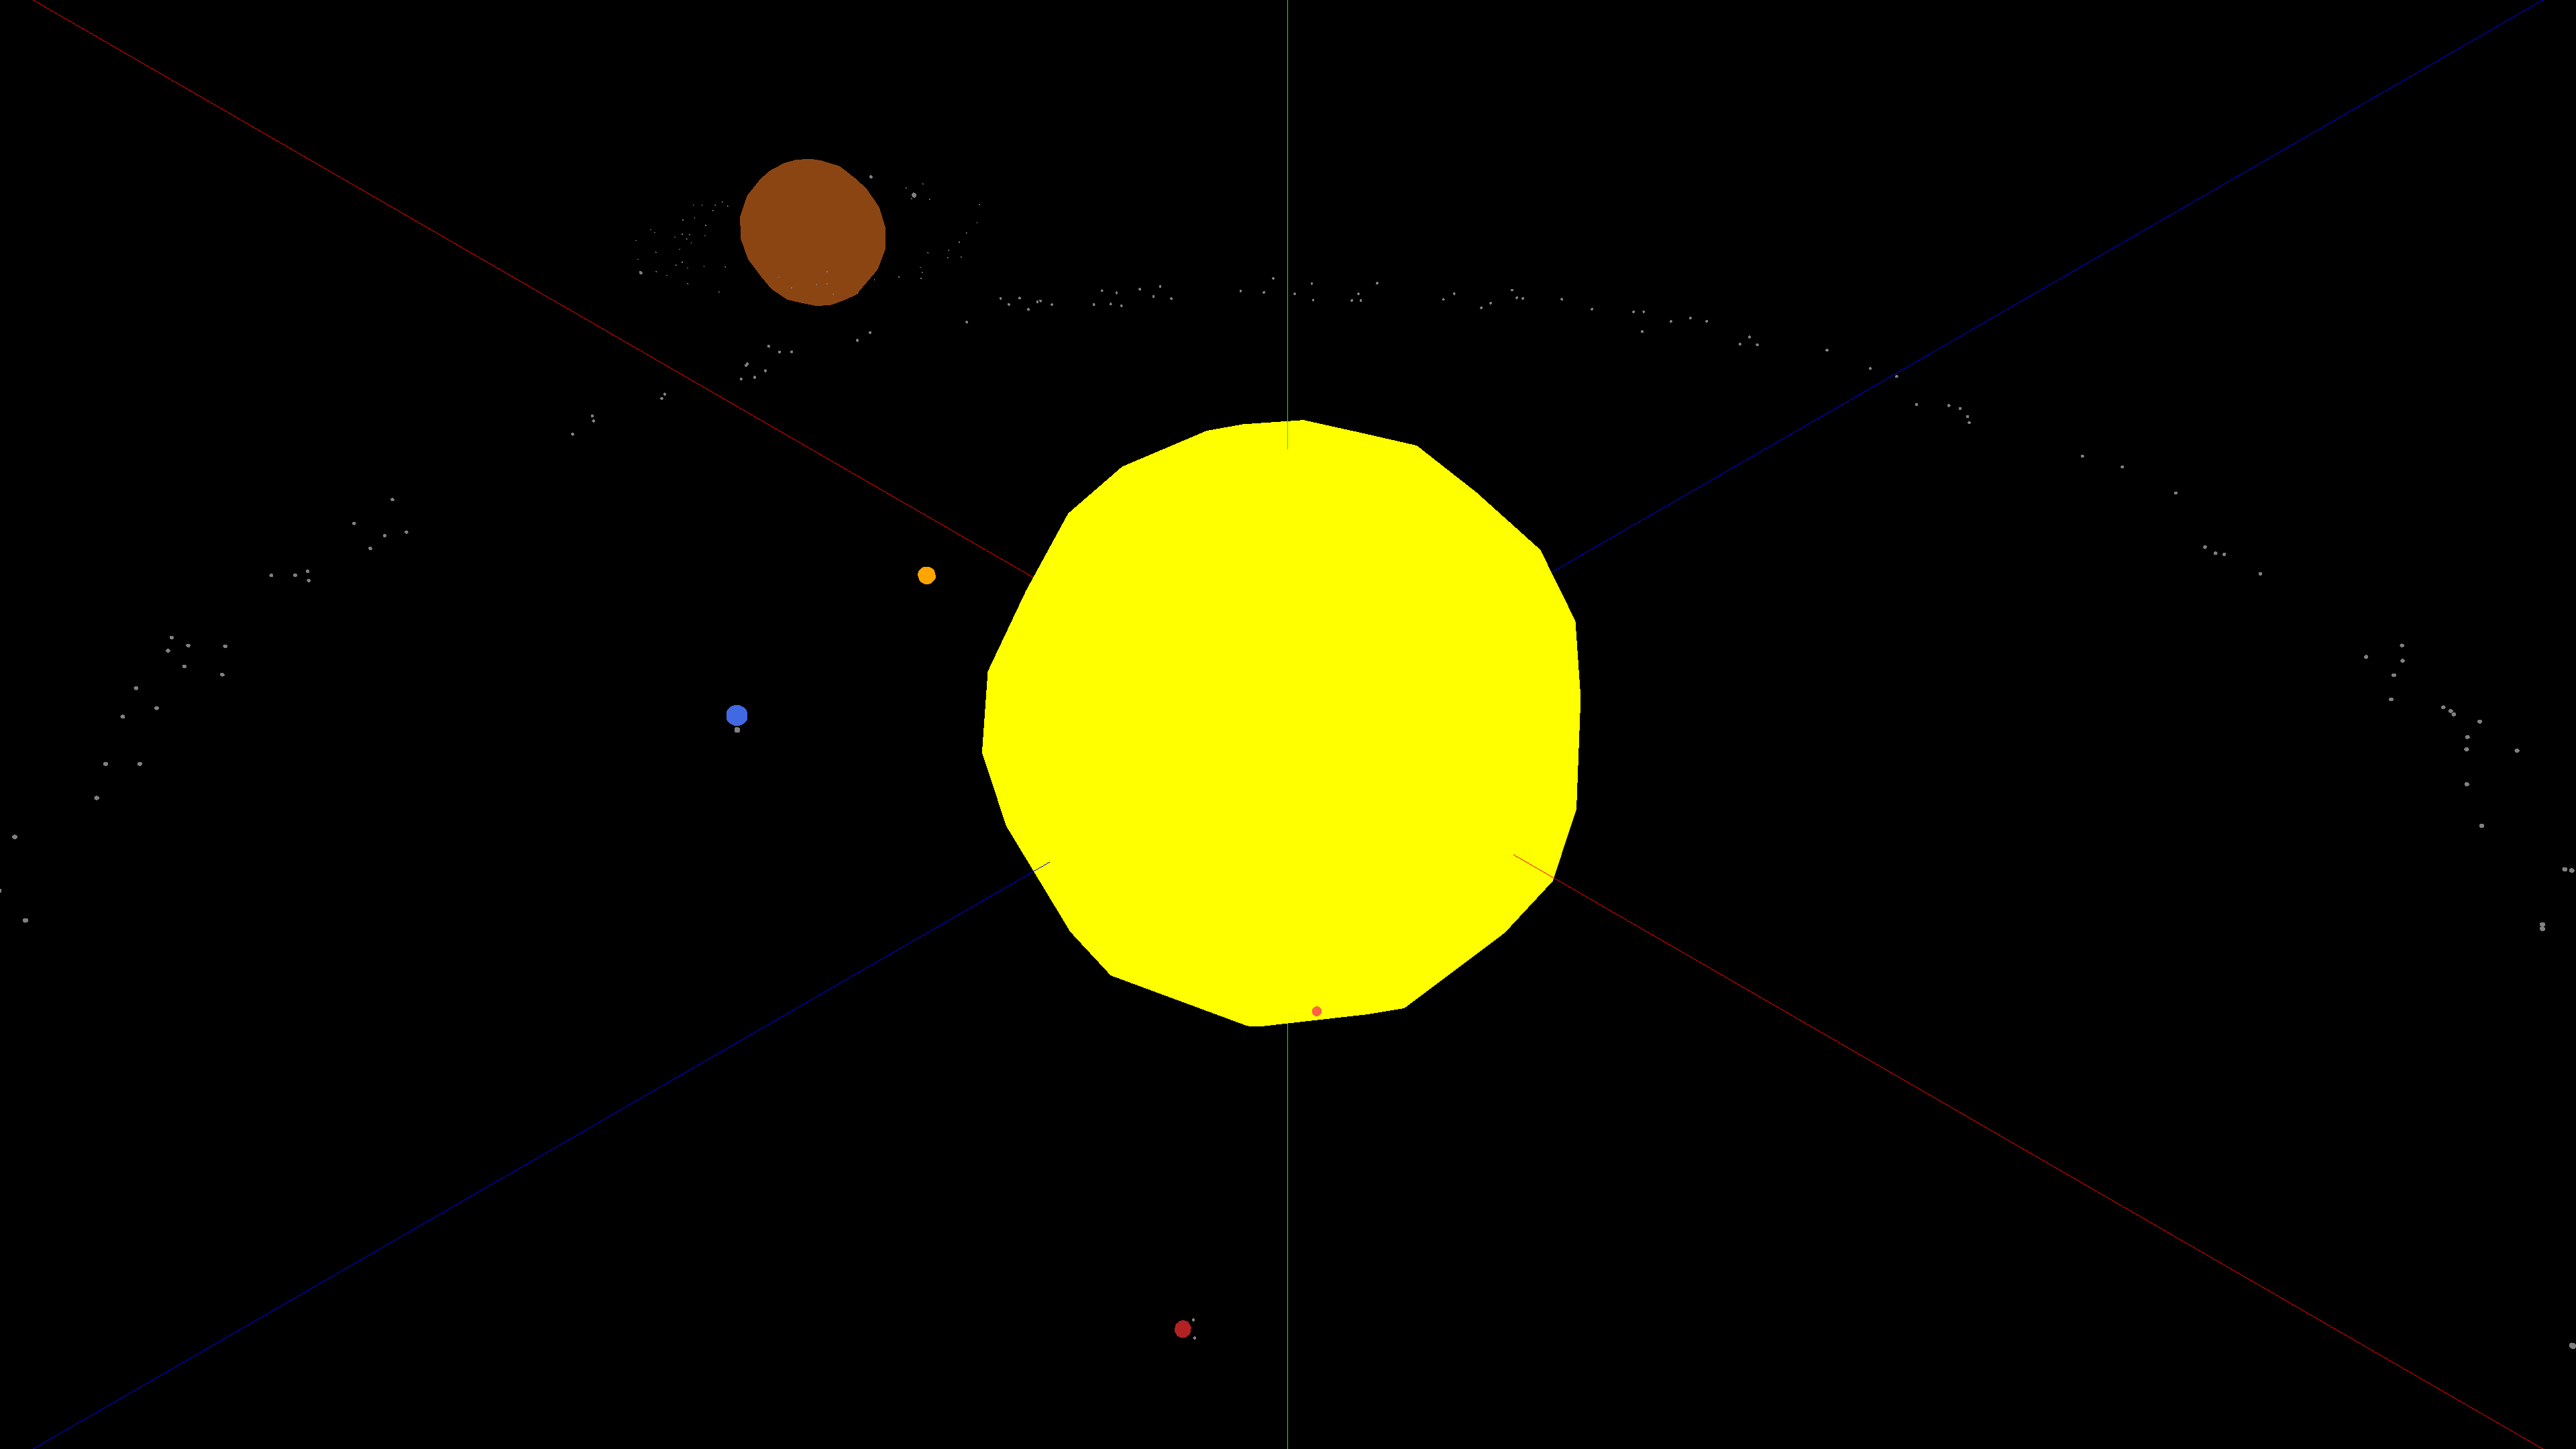
\includegraphics[width=\textwidth]{images/axis.png}
                \caption{com eixos}
            \end{minipage}
        \end{figure}
    \item \textit{g}: toggle debug mode
        \subitem toggle eixos
        \subitem toogle ponto para onde a camera está a olhar (a verde)
        \subitem toggle fps counter (no nome da janela)
        \begin{figure}[H]
            \centering
            \begin{minipage}{0.49\textwidth}
                \centering
                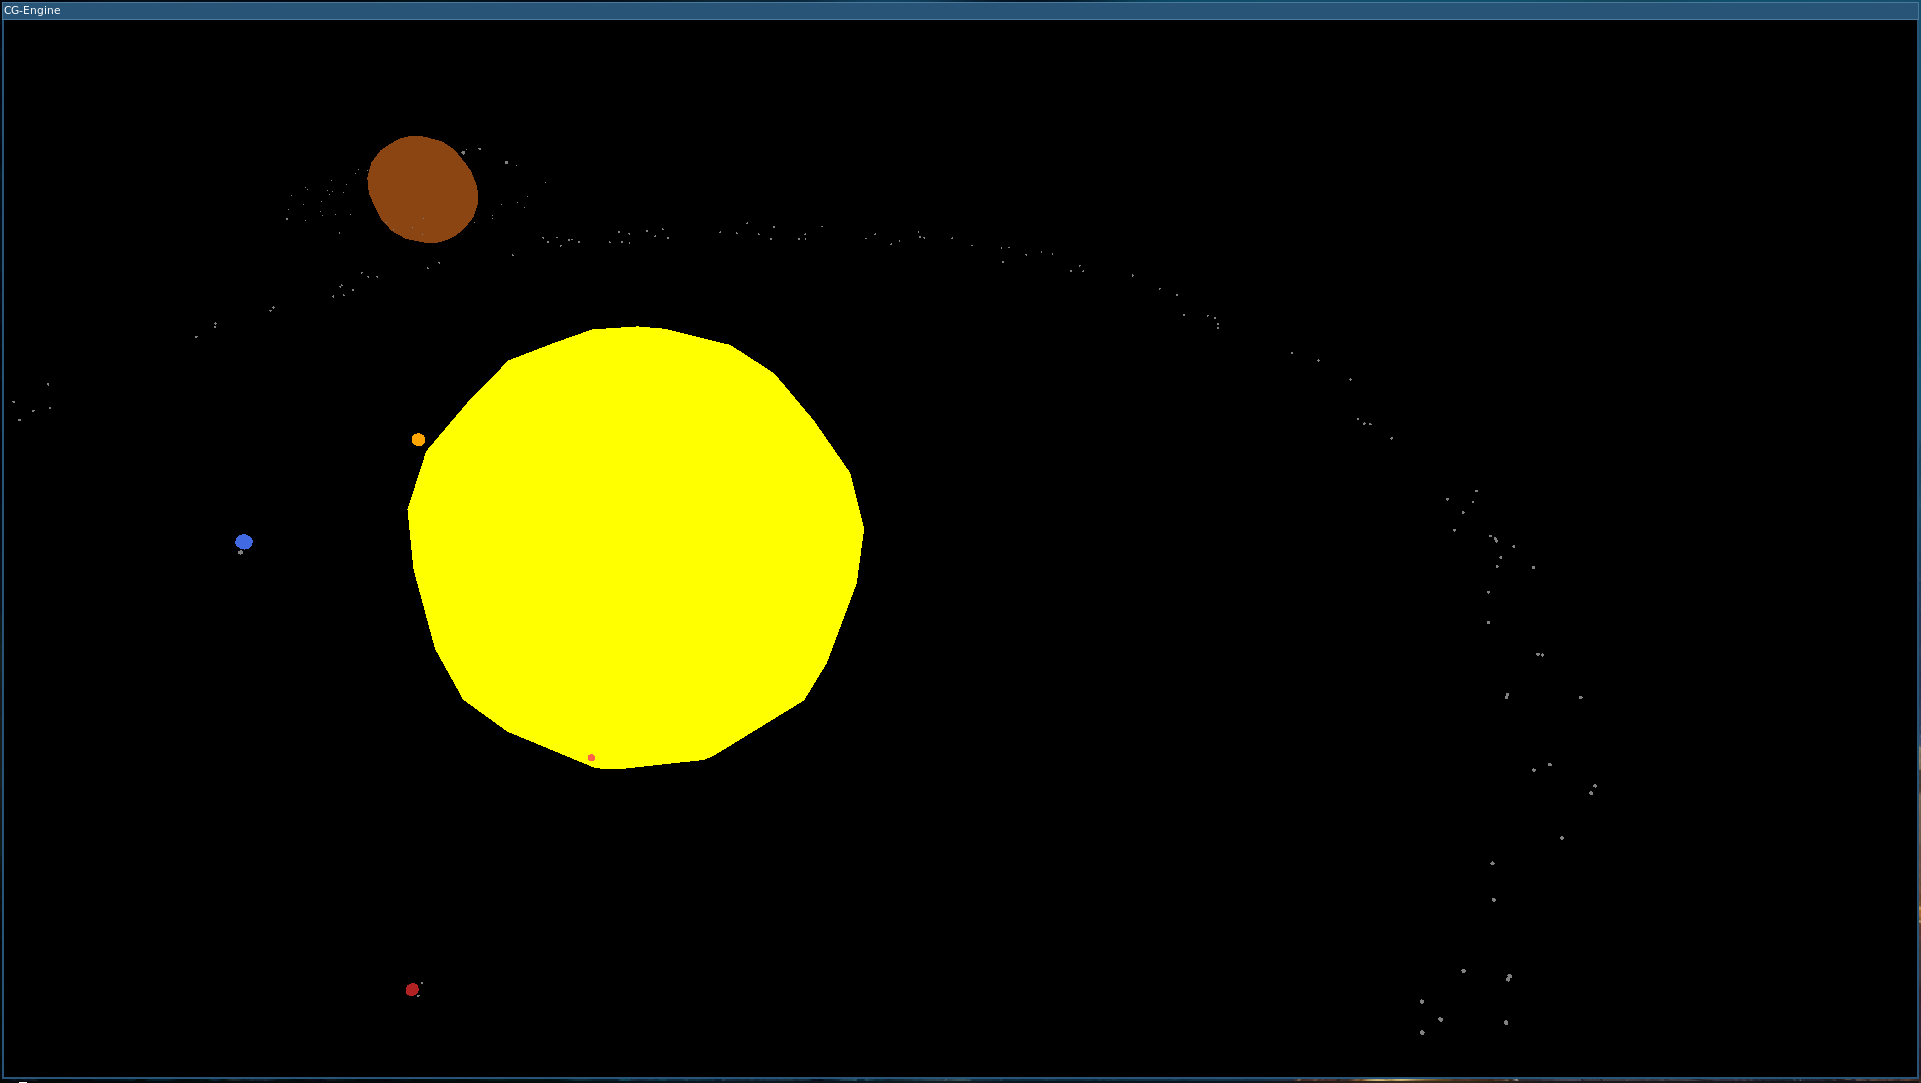
\includegraphics[width=\textwidth]{images/normal_mode.png}
                \caption{modo normal}
            \end{minipage}\hfill
            \begin{minipage}{0.49\textwidth}
                \centering
                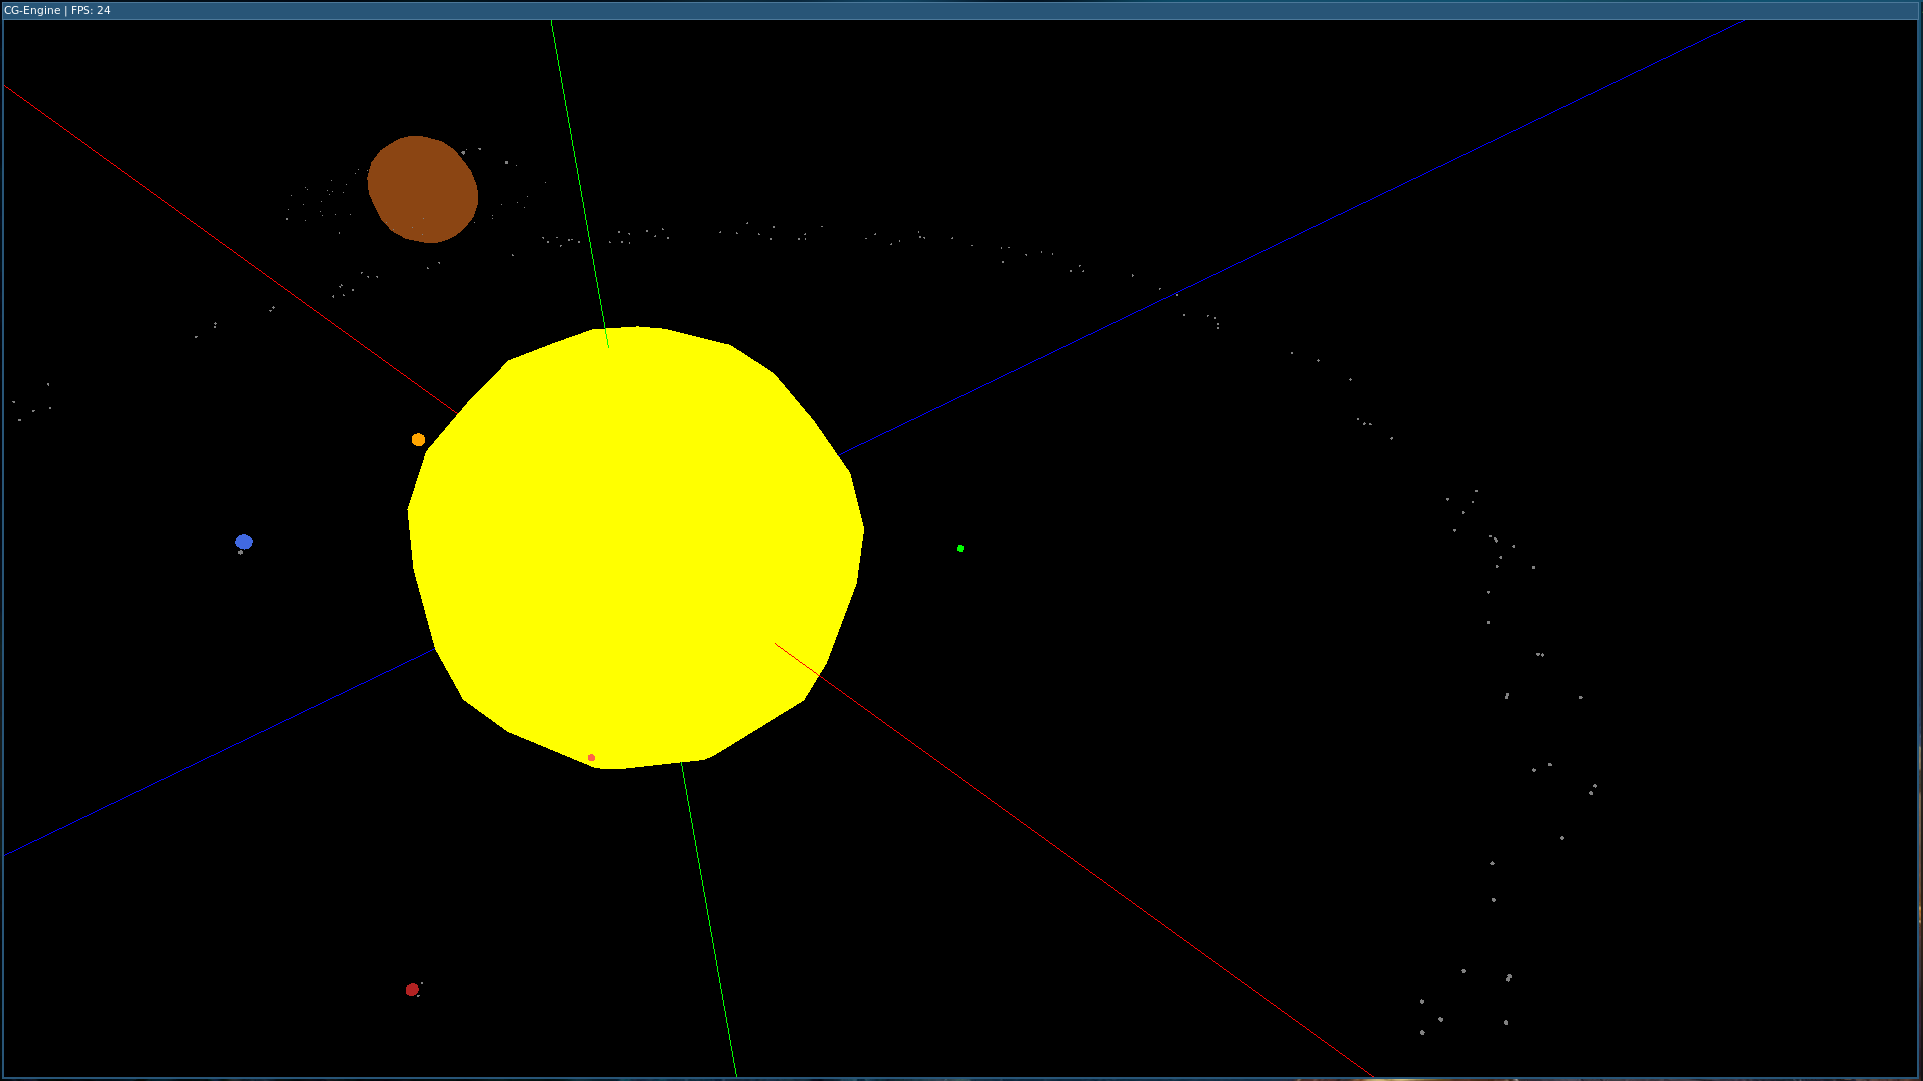
\includegraphics[width=\textwidth]{images/debug_mode.png}
                \caption{modo debug}
            \end{minipage}
        \end{figure}
\end{itemize}

\chapter{Generator}
Neste módulo foram definidas na fase anterior 5 primitivas:
\begin{itemize}
        \item Plano
        \item Caixa
        \item Esfera
        \item Cone
        \item Cilindro
\end{itemize}
Nesta fase implementamos uma nova primitiva, o Torus.\\

\section{Torus}
Para desenhar uma Torus é preciso saber o raio interior de uma torus, o raio
exterior, o número de stacks(\textit{\_stacks} e o número de
slices(\textit{\_slices}).\\
Para facilitar os cálculos estes valores são internamente convertidos para o
raio que vai do centro da torus ao centro do anel da torus (\textit{\_radius}) e
o raio do anel propriamente dito (\textit{\_ring\_radius}).

\begin{figure}[H]
    \centering 
    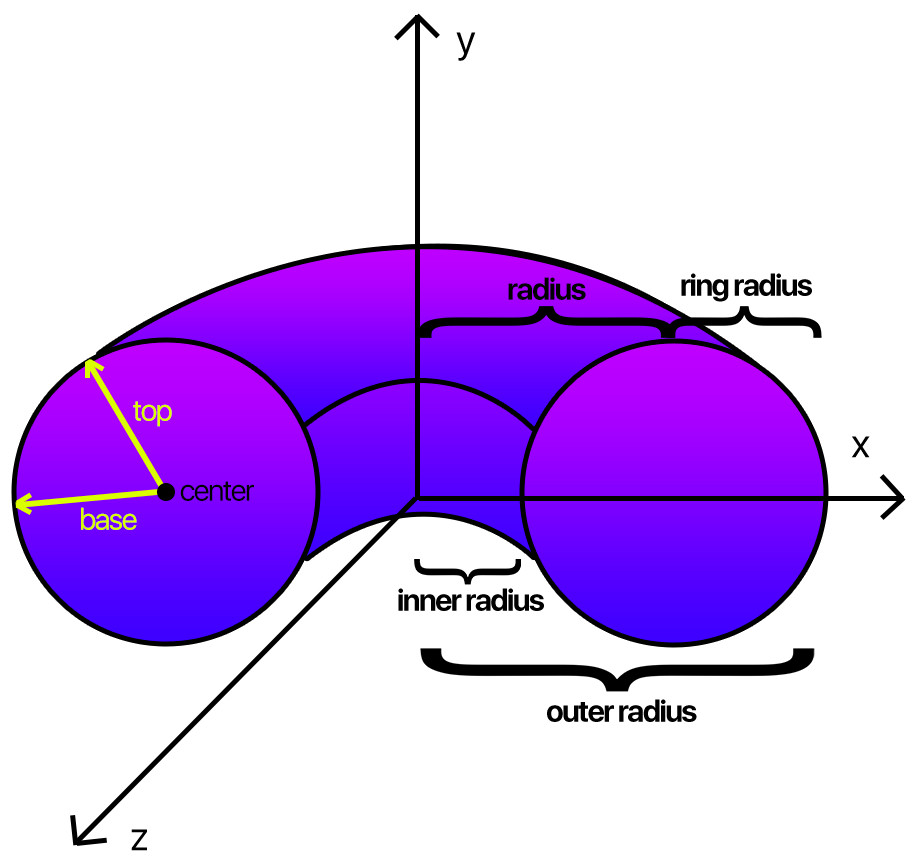
\includegraphics[width=0.5\textwidth]{images/torus_points.png}
    \caption{Esquema dos pontos no plano}
    \label{fig:scheme_torus}
\end{figure}
Primeiro é definido o ângulo entre cada slice e cada stack com:
\begin{lstlisting}
float ang\_slice = 2.0f * M\_PI / \_slices;
float ang\_stack = 2.0f * M\_PI / \_stacks;
\end{lstlisting}
Em seguida, percorremos todas as slices e stacks com dois ciclos for aninhados.
em cada ciclo são calculados dois pontos e quatro vetores.\\

\begin{lstlisting}
auto   center = PointSpherical(_radius, M_PI/2.0f, ang_slice * slice);
auto n_center = PointSpherical(_radius, M_PI/2.0f, ang_slice * (slice+1));
\end{lstlisting}
O ponto \textit{center} é um ponto dentro do aro em si e que vai andando ao
longo do centro do aro. o ponto \textit{n\_center} é exatamente o mesmo que o
ponto calculado anteriormente mas imediatamente a seguir.

\begin{lstlisting}
auto base = VectorSpherical(_ring_radius, ang_stack *  stack, center.azimuth());
auto top = VectorSpherical(_ring_radius, ang_stack * (stack + 1), center.azimuth());
auto n_base = VectorSpherical(_ring_radius, ang_stack *  stack, n_center.azimuth() );
auto n_top = VectorSpherical(_ring_radius, ang_stack * (stack + 1), n_center.azimuth() );
\end{lstlisting}
O vetor \textit{base} vai desde o ponto no centro do aro até à borda do aro.\\
Assim, para obter todos os pontos na face do torus basta percorrer todos os
valores de slice e stack e para cada um somar o ponto \textit{center} ao vetor
\textit{base}.\\
Visto que é necessário obter triângulos, precisamos de saber outros pontos em
torno do ponto calculado.\\
Assim, o vetor \textit{top} aponta para o ponto imediatamente acima do ponto
calculado com o vetor \textit{base}, o vetor \textit{n\_base} aponta para o
ponto ao lado e o vetor \textit{n\_top} aponta para o ponto imediatamente acima
e ao lado.\\
Logo para calcular todos os pontos por ordem utilizamos o seguinte código:

\begin{lstlisting}
for(i32 slice = 0; slice < _slices; slice++) {
    for(i32 stack = 0; stack < _stacks; stack++) {
        // 1st triangle
        coords.push_back(  center + top);
        coords.push_back(n_center + n_base);
        coords.push_back(  center + base);

        //2nd triangle
        coords.push_back(  center + top);
        coords.push_back(n_center + n_top);
        coords.push_back(n_center + n_base);
    }
}
\end{lstlisting}

\begin{figure}[H]
    \centering 
    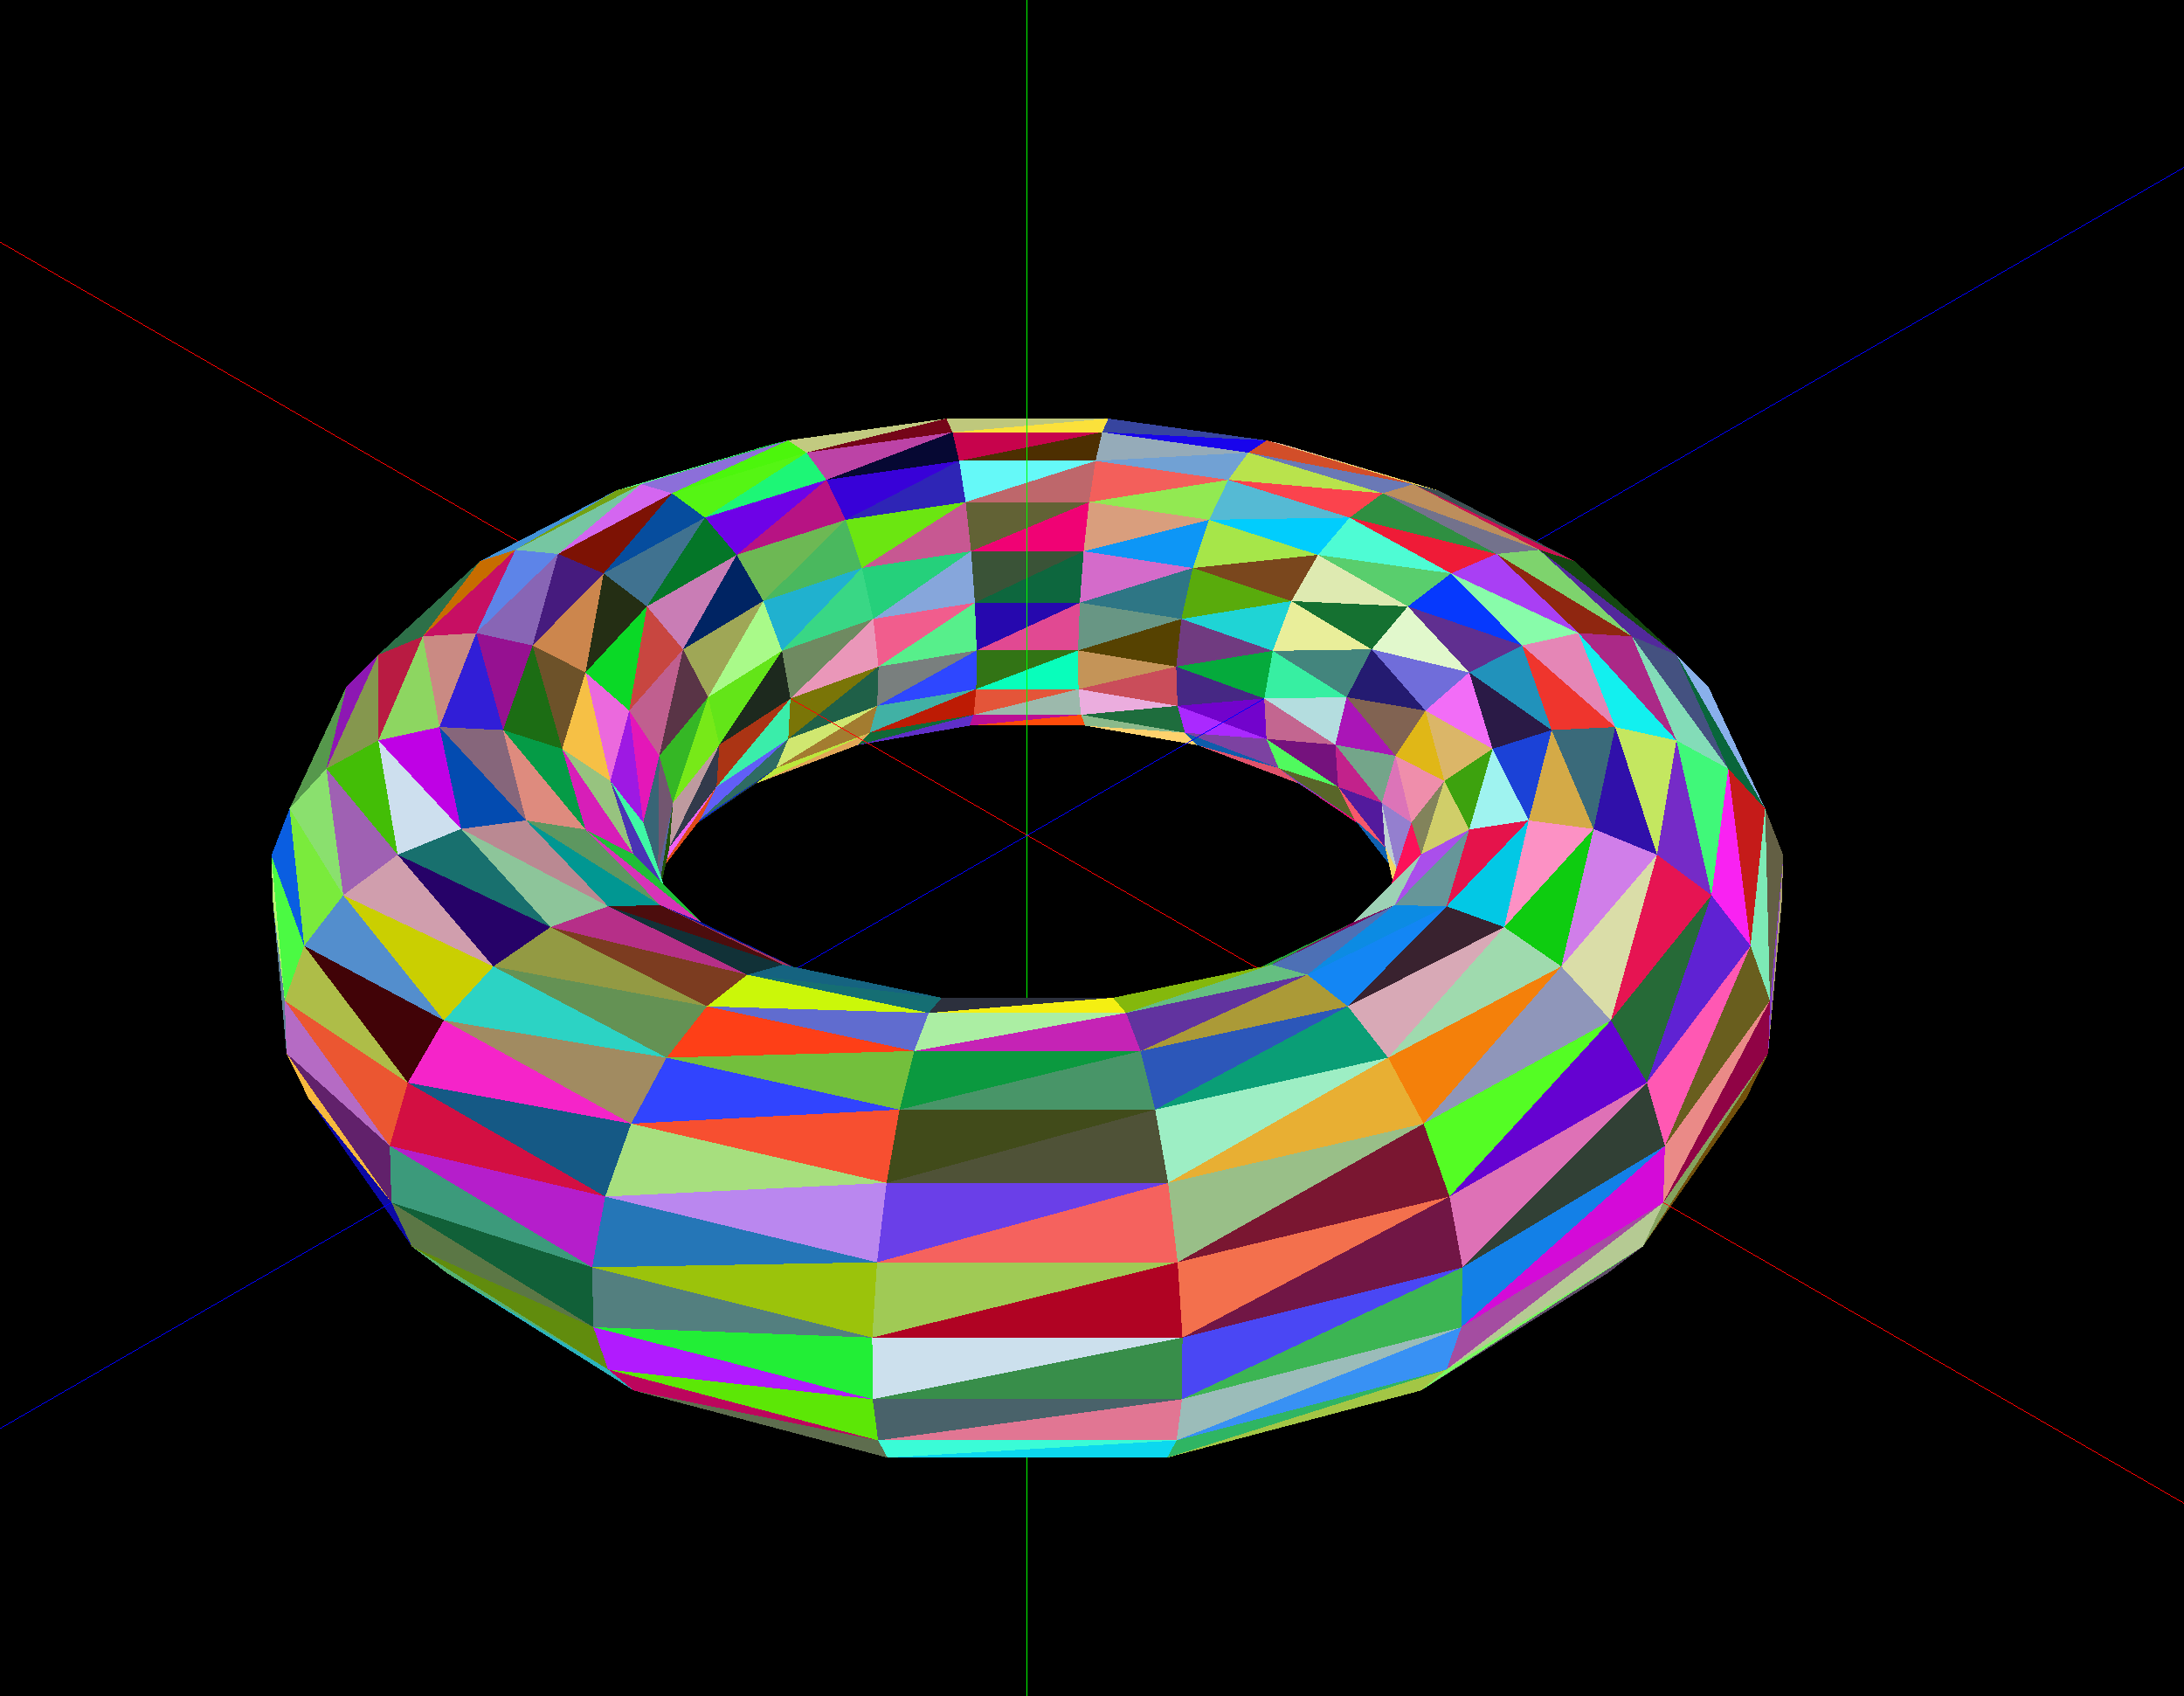
\includegraphics[width=0.5\textwidth]{images/torus.png}  
    \caption{Torus: inner radius:1 outer radius:2 slices:20 stacks:20}
    \label{fig:torus_render}
\end{figure}

\chapter{Solar System}
Para facilitar desenhar o sistema solar decidimos criar um script em Python.\\
De forma a criar um modelo relativamente realista do sistema solar decidimos
seguir um conjunto de regras simples.

\begin{itemize}
        \item tamanho de planetas e luas está à escala entre planetas e luas
        \item distancia dos planetas e cinturas de asteróides ao sol está à
            escala dentro de si próprio
\end{itemize}
Criando várias escalas permite que seja criado um modelo relativamente realista
do sistema solar mas ao mesmo tempo visualmente apelativo.\\
A informação sobre a distancia relativa dos planetas ao sol veio do
\textit{National Geographic} (
\url{https://www.nationalgeographic.org/activity/planetary-size-and-distance-comparison/})
e foram colocados dentro de um csv com mais alguma informação, tal como, se o
planeta tem um sistema de anéis ou não.\\
A informação sobre as luas presentes no sistema solar foi obtida de um CSV
publicamente disponivel em
\url{https://github.com/devstronomy/nasa-data-scraper/blob/master/data/csv/satellites.csv}.
Com base nestes dois ficheiros, é possível desenhar um sistema solar com mais de
100 luas.\\
Por fim decidimos acrescentar a cintura de asteróides e a cintura de
\textit{Kuiper} com 200 e 1000 asteróides respectivamente.\\

\begin{figure}[H]
    \centering 
    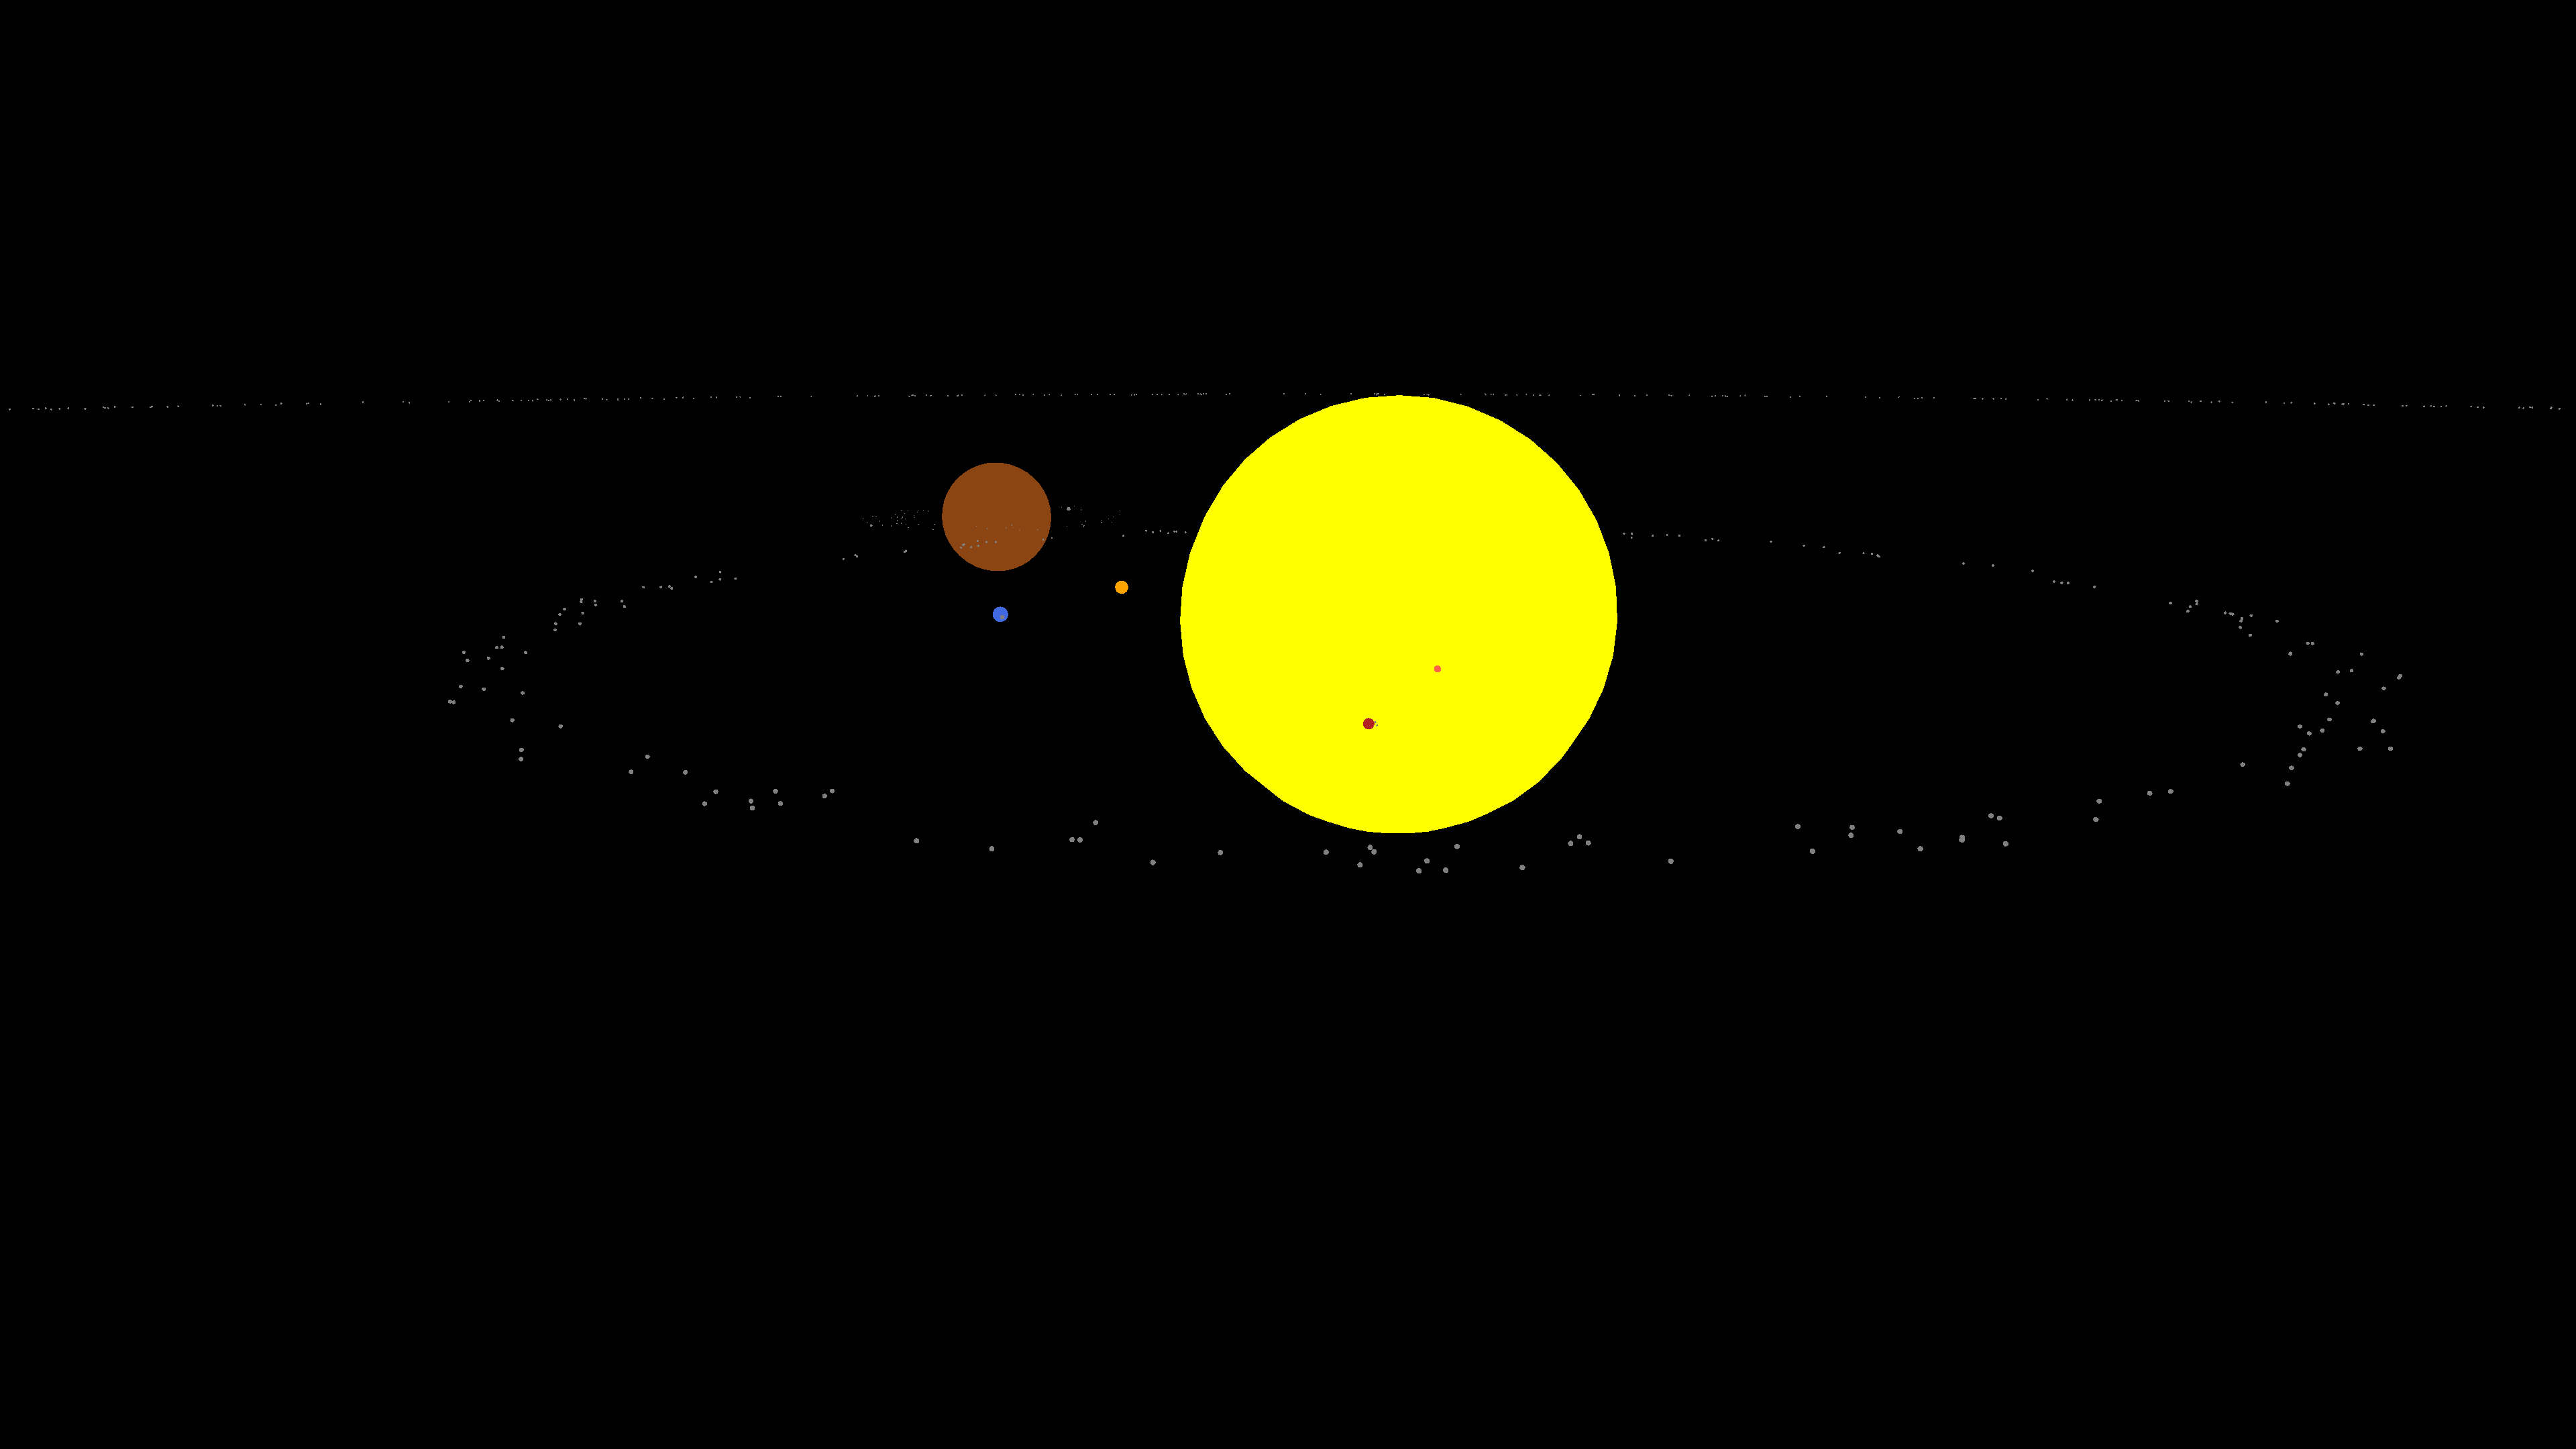
\includegraphics[width=0.8\textwidth]{images/sun.png}  
    \caption{Imagem do sol}
    \label{fig:sun}
\end{figure}
\begin{figure}[H]
    \centering 
    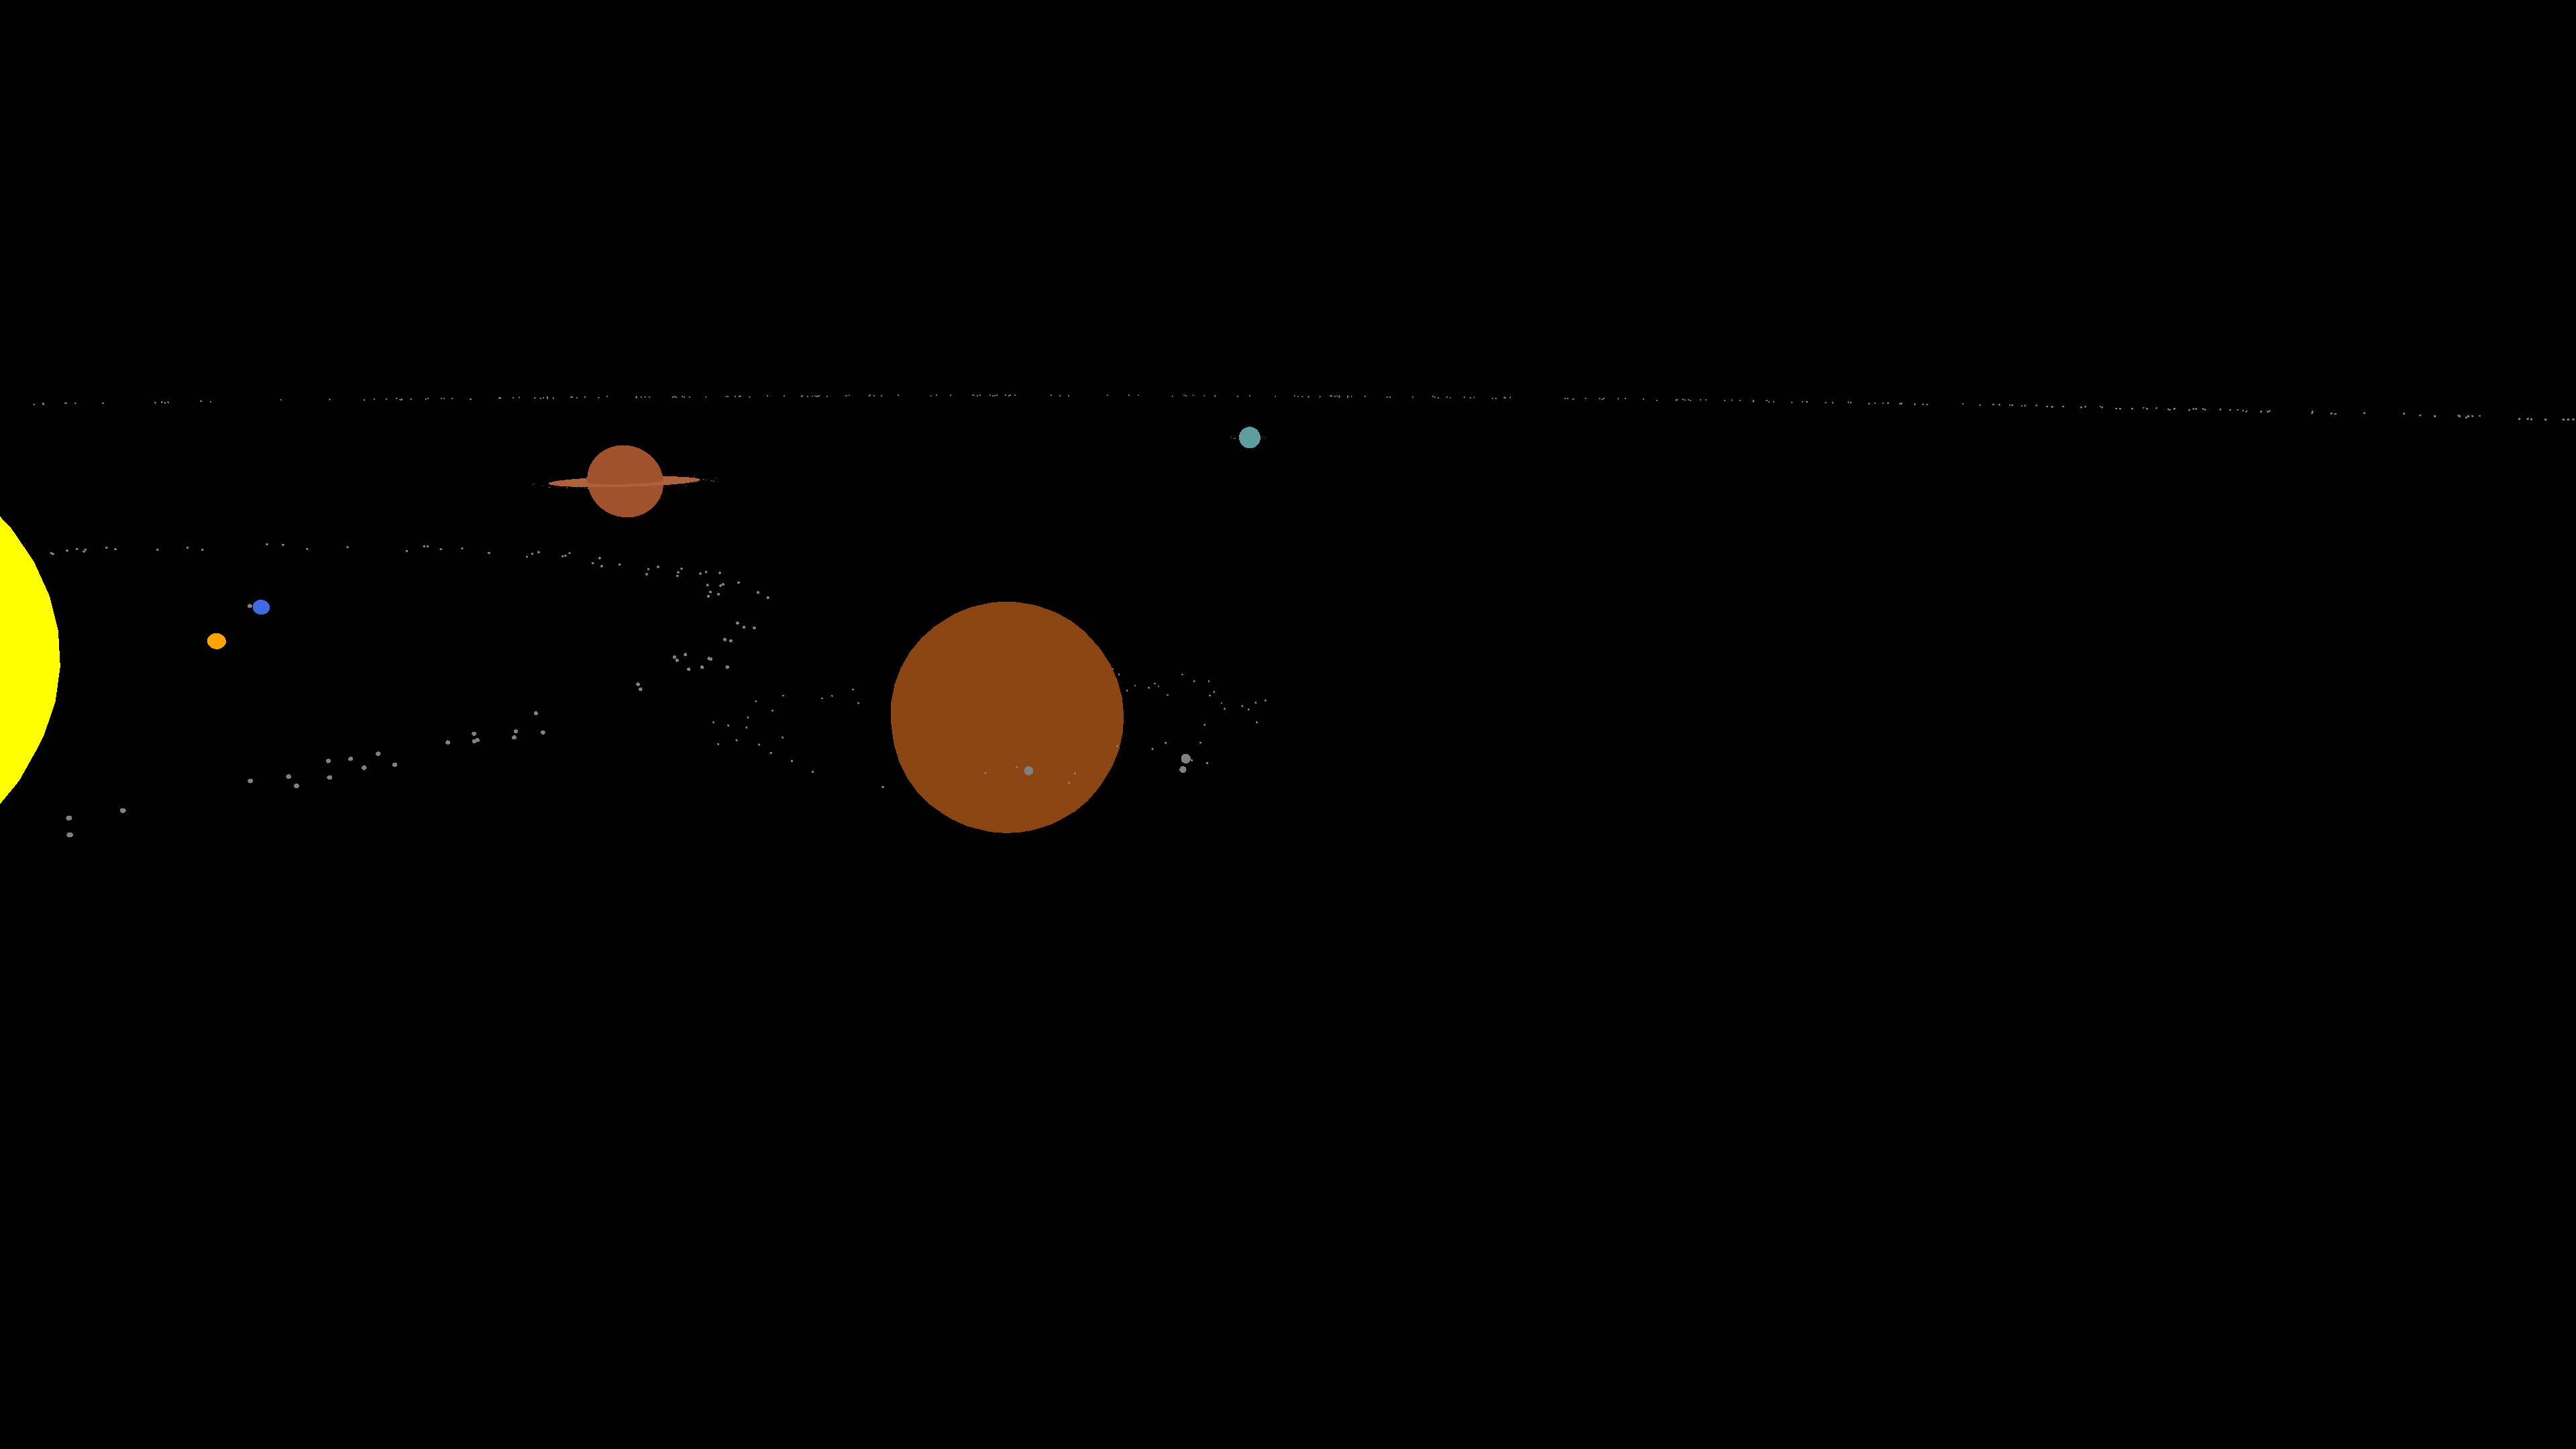
\includegraphics[width=0.8\textwidth]{images/jupiter.png}  
    \caption{Imagem de Júpiter e as suas luas}
    \label{fig:jupiter}
\end{figure}
\begin{figure}[H]
    \centering 
    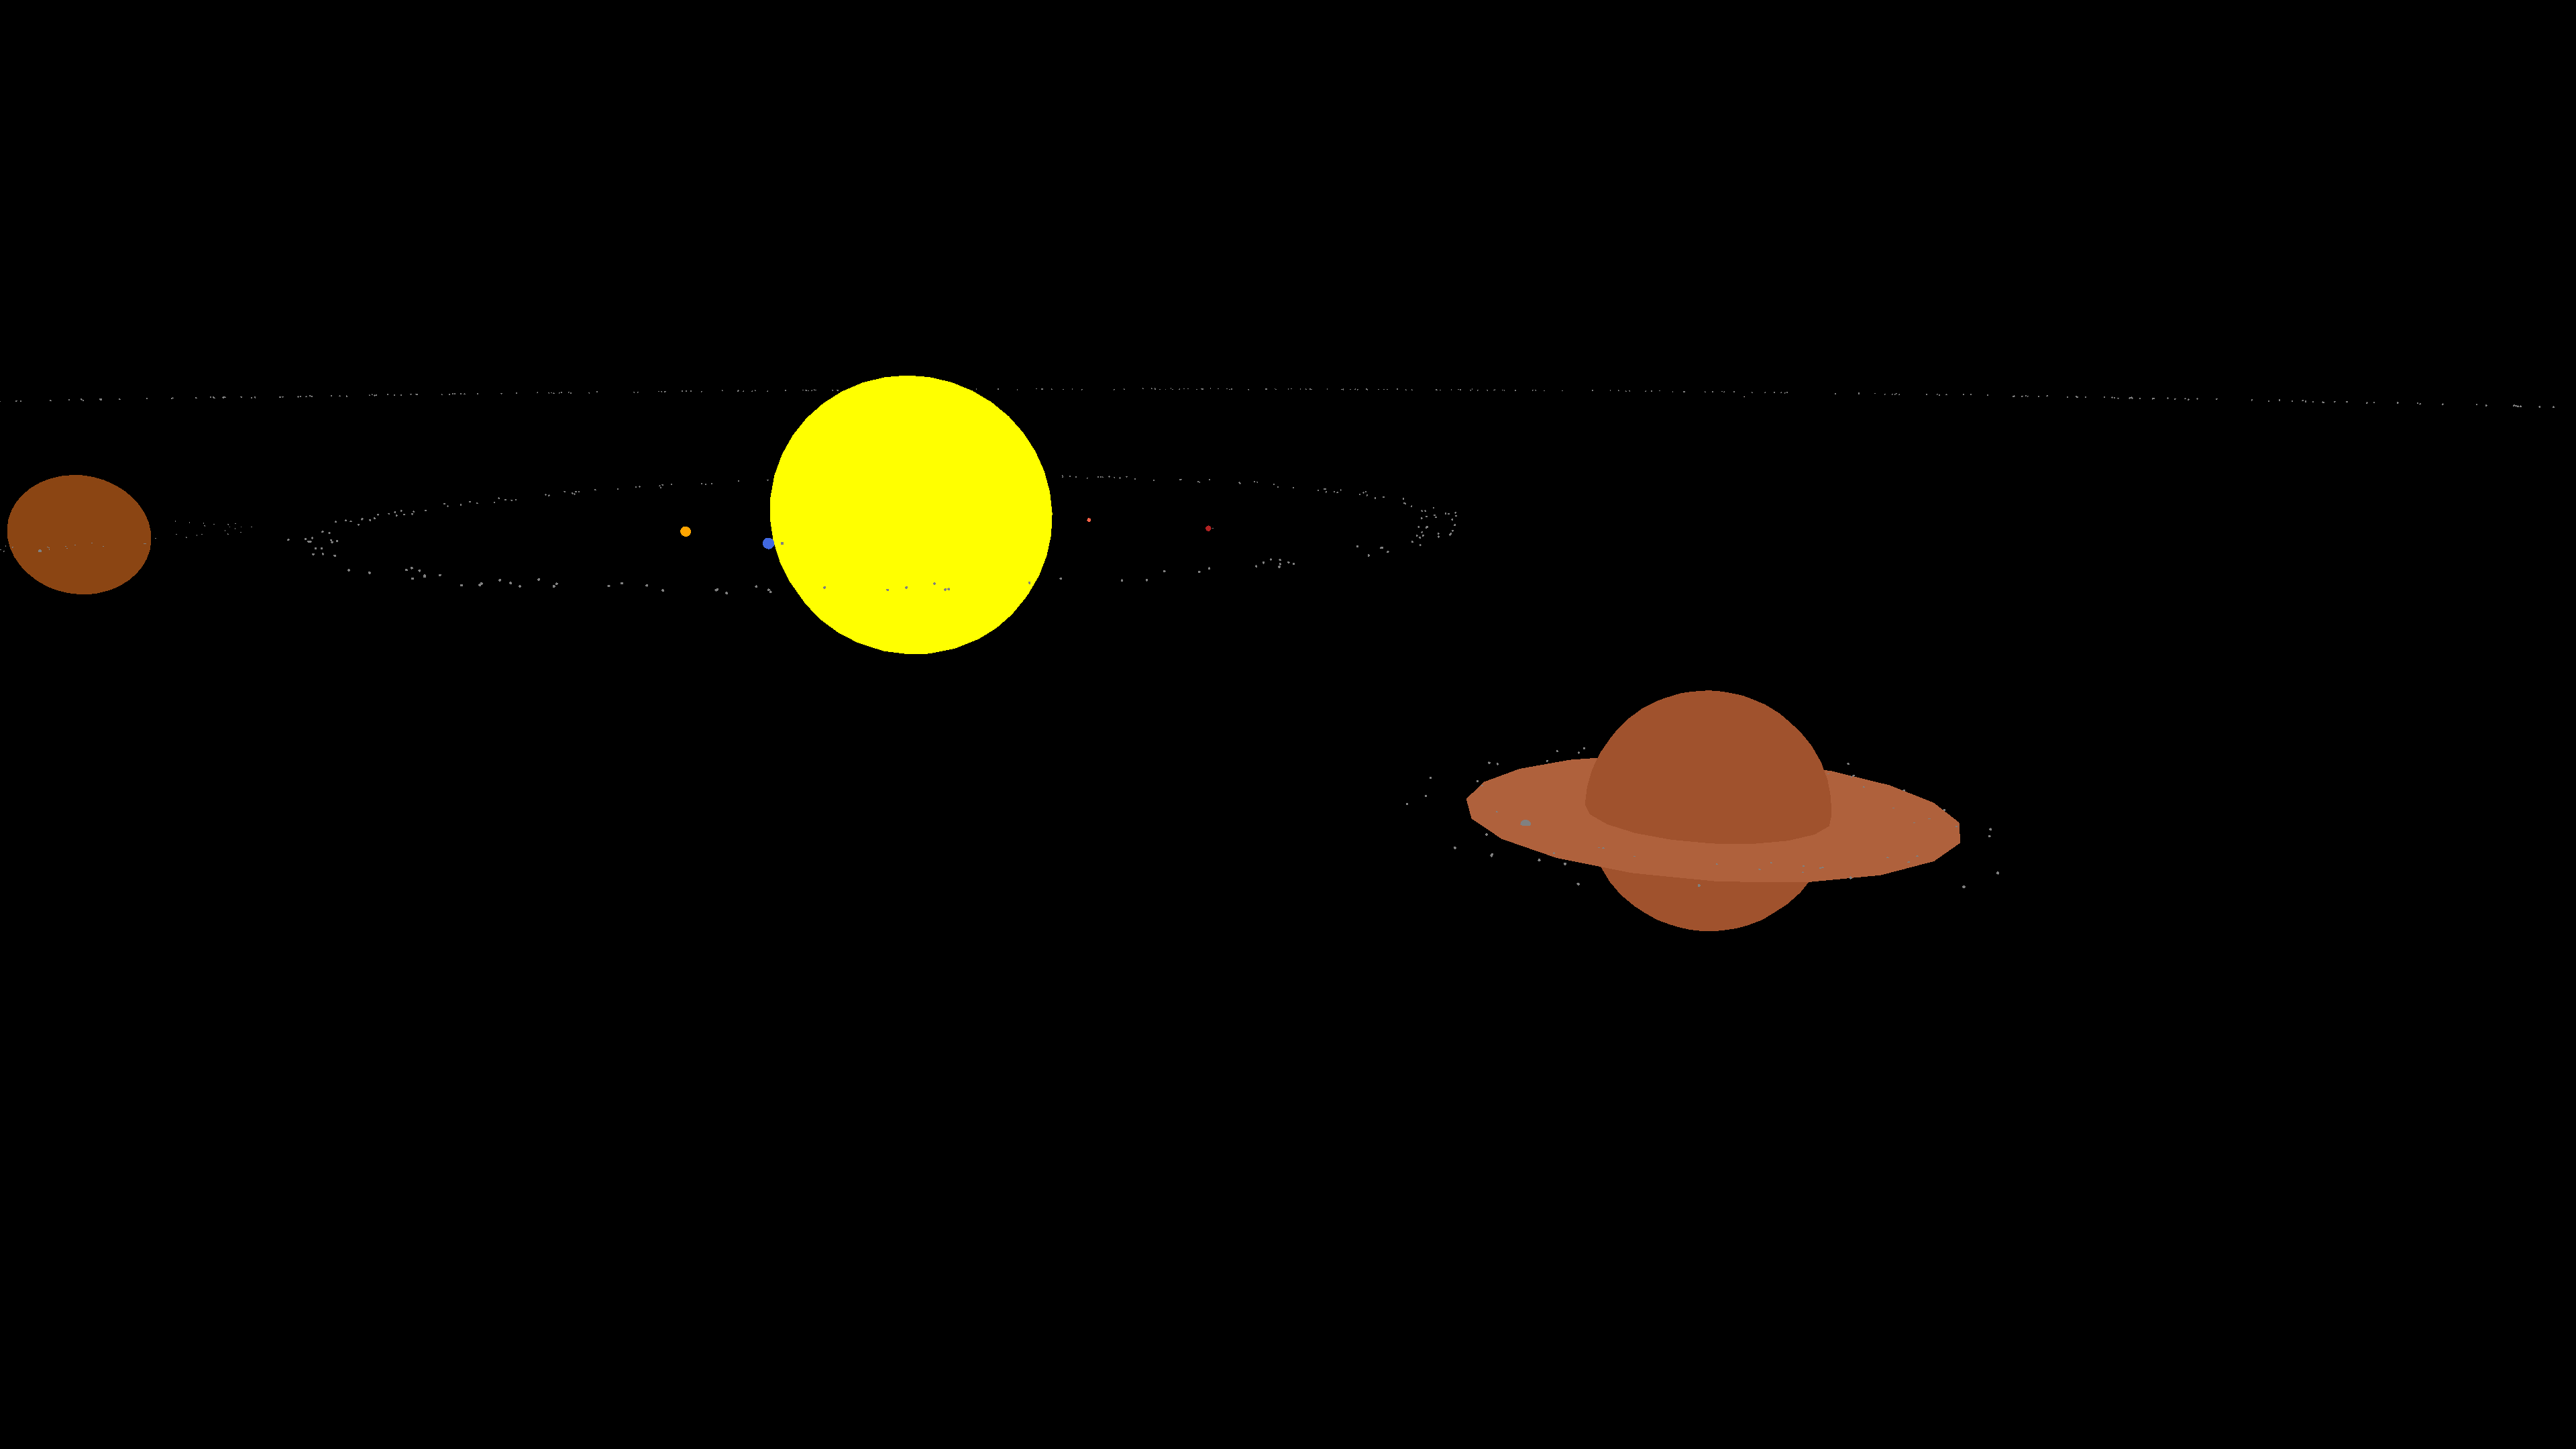
\includegraphics[width=0.8\textwidth]{images/saturno.png}  
    \caption{Imagem de Saturno}
    \label{fig:saturn}
\end{figure}

\chapter{Conclusão}
Com este trabalho prático podemos aplicar os conhecimentos lecionados até agora
nas aulas da unidade curricular de computação gráfica permitindo assim que
aprofundar os nossos conhecimentos de openGl.\\
Como trabalho futuro gostaríamos de criar mais scenes para testar as capacidades
do nosso \textit{Engine}, implementar animações e melhorar a performance do
nosso engine com recurso a VBOs.

\end{document}
